\documentclass{article}
\usepackage[utf8]{inputenc}
\usepackage{amsmath}
\usepackage{amssymb}
\usepackage{parskip}
\usepackage{fullpage}
\usepackage{hyperref}
\usepackage{multirow}
\usepackage{listings}
\usepackage{makecell}
\usepackage{color}
\usepackage{xcolor}
\usepackage{graphicx}
\usepackage{multicol}
\usepackage[backend=bibtex]{biblatex} % texlive-bibtexextra

\hypersetup{
    colorlinks=true,
    linkcolor=black,
    urlcolor=blue,
    pdftitle={Fourier Analysis Documentation},
    pdfpagemode=FullScreen,
}

%\newacronym{dft}{DFT}{Discrete Fourier Transform}
%\newacronym{fft}{FFT}{Fast Fourier Transform}
%\newacronym{fs}{FS}{Fourier Series}
%\newacronym{ft}{FT}{Fast Transform}
%\makeglossary

\definecolor{lightgray}{rgb}{0.9,0.9,0.9}
\definecolor{darkgray}{rgb}{0.2,0.4,0.2}
\definecolor{darkgreen}{rgb}{0.0,0.4,0.0}
\definecolor{olive}{rgb}{0.17,0.59,0.20}

\lstdefinelanguage{JavaScript}{
    keywords={typeof, new, true, false, catch, function, return, null, catch, switch, var, if, in, while, do, else, case, break},
    keywordstyle=\color{blue}\bfseries,
    ndkeywords={class, extends, export, boolean, throw, implements, import, this},
    ndkeywordstyle=\color{olive}\bfseries,
    sensitive=false,
    comment=[l]{//},
    morecomment=[s]{/*}{*/},
    commentstyle=\color{darkgray}\ttfamily,
    morestring=[b]',
    morestring=[b]",
    stringstyle=\color{red}\ttfamily
}

\lstdefinestyle{js} {
   language=JavaScript,
   backgroundcolor=\color{lightgray},
   extendedchars=true,
   basicstyle=\footnotesize\ttfamily,
   showstringspaces=false,
   showspaces=false,
   numberstyle=\footnotesize,
   numbersep=9pt,
   tabsize=2,
   breaklines=true,
   showtabs=false,
   captionpos=b
}

\lstdefinelanguage{HTML5}{
    keywords={head, body, div, ul, ol, lh, li, table, input, meta, title, thead, tbody, tr, th, pre, p, nav, main, header, h1, h2, h3, h4, h5, h6, footer, i, b, u, style, link, img, q},
    keywordstyle=\color{blue}\bfseries,
    sensitive=false,
    comment=[s]{<!--}{-->},
    commentstyle=\color{darkgray}\ttfamily,
    morestring=[b]",
    stringstyle=\color{red}\ttfamily
}

\lstdefinestyle{html} {
   language=HTML5,
   backgroundcolor=\color{lightgray},
   extendedchars=true,
   basicstyle=\footnotesize\ttfamily,
   showstringspaces=false,
   showspaces=false,
   numberstyle=\footnotesize,
   numbersep=9pt,
   tabsize=2,
   breaklines=true,
   showtabs=false,
   captionpos=b
}

\graphicspath{ {./img/} }
\addbibresource{references.bib}

\newcommand{\tabitem}{~~\llap{\textbullet}~~}

\title{Fourier Analysis}

\title{%
  Fourier Analysis \\
  \large Documentation}

\author{%
    Paolo Bettelini \\
    \large Scuola d'Arti e Mestieri di Trevano (SAMT)}

\date{}

\begin{document}

\maketitle

\pagebreak

\tableofcontents

\pagebreak

\section{Introduction}

\subsection{Abstract}

Fourier analysis is a method of defining periodic waveforms in terms of trigonometric functions.
This branch of mathematics is widely used in signal processing, especially electronics, acoustics and communications.
Many notorious algorithms have been developed thanks to Joseph Fourier. Operators such as the Fourier
Transform are constantly used in the real world, without these discoveries the world would not be the same.
Much software relies in Fourier Analysis, such as for instance Shazam, the famous service for identifying songs.
Any audio spectrum visualized processes the signal using Fourier Transform, these are just a few of the many application of this analysis.

\pagebreak

\subsection{Informations}

This is a project of the Scuola Arti e Mestieri di Trevano (SAMT) under the following circumstances

\begin{itemize}
    \item \textbf{Section}: Computer Science
    \item \textbf{Year:} Third
    \item \textbf{Class:} Module 306
    \item \textbf{Supervisor:} Luca Muggiasca
    \item \textbf{Title:} Fourier Analysis
    \item \textbf{Start date}: 2021-09-09
    \item \textbf{Deadline}: 2021-12-23
\end{itemize}

and the following requirements

\begin{itemize}
    \item \textbf{Documentation}: a full documentation of the work done
    \item \textbf{Changelog}: constant changelog for each work session
    \item \textbf{Source code}: working source code of the project
\end{itemize}

All the source code and documents can be found at \href{https://github.com/paolobettelini/fourier-series}{https://github.com/paolobettelini/fourier-series}\cite{gitrepo}.
\\
The live version of the final product is available at \href{https://paolobettelini.github.io/fourier-series}{https://paolobettelini.github.io/fourier-series}\cite{gitpages}.

\subsection{Scope}

The scope of this project is to create a website containing various explanations about Fourier Analysis. \\
The website must be able to explain the various concepts in a comprehensible way and with interactive and visual examples.

\pagebreak

\section{Analysis}

\subsection{Analysis of the means}

\begin{itemize}
    \item Firefox (95.0+) as browser
    \item GitHub\cite{github} as code repository
    \item Visual Studio Code as IDE
    \item PdfLaTeX as LaTeX to PDF renderer
    \item Instagantt\cite{instagantt} as project management software
\end{itemize}

\subsection{Requirements Analysis}

\subsubsection{Req-00}

\bgroup{}
\def\arraystretch{1.25}
\begin{center}
    \begin{tabular}{ |l|p{9cm}| }
        \hline
        \multicolumn{2}{|c|}{\textbf{Req-00}} \\
        \hline
        \textbf{Name} & Content \\
        \hline
        \textbf{Priority} & 1 \\
        \hline
        \textbf{Version} & 2.0 \\
        \hline
        \textbf{Notes} & none \\
        \hline
        \textbf{Description}
        & The website must contains a full explanation about Fourier Analysis. \\
        \hline
    \end{tabular}
\end{center}
\egroup{}

\subsubsection{Req-01}

\bgroup{}
\def\arraystretch{1.25}
\begin{center}
    \begin{tabular}{ |l|p{9cm}| }
        \hline
        \multicolumn{2}{|c|}{\textbf{Req-01}} \\
        \hline
        \textbf{Name} & Index \\
        \hline
        \textbf{Priority} & 1 \\
        \hline
        \textbf{Version} & 2.0 \\
        \hline
        \textbf{Notes} & none \\
        \hline
        \textbf{Description}
        & The website must contain an index of all the sections \\
        \hline
        \multicolumn{2}{|c|}{\textbf{Subrequirements}} \\
        \hline
        \textbf{Req-01\_0} & There must be a section about the topic introduction. \\
        \hline
        \textbf{Req-01\_1} & There must be a section about the knowledge requirements. \\
        \hline
        \textbf{Req-01\_2} & There must be a section about signal processing. \\
        \hline
        \textbf{Req-01\_3} & There must be a section about the Fourier transform. \\
        \hline
        \textbf{Req-01\_4} & There must be a section about the Fourier series. \\
        \hline
        \textbf{Req-01\_5} & There must be a section about how to represent the Fourier series with epicycles. \\
        \hline
        \textbf{Req-01\_6} & There must be a section about Fast Fourier Transform. \\
        \hline
    \end{tabular}
\end{center}
\egroup{}

\subsubsection{Req-02}

\bgroup{}
\def\arraystretch{1.25}
\begin{center}
    \begin{tabular}{ |l|p{9cm}| }
        \hline
        \multicolumn{2}{|c|}{\textbf{Req-02}} \\
        \hline
        \textbf{Name} & Responsiveness \\
        \hline
        \textbf{Priority} & 1 \\
        \hline
        \textbf{Version} & 1.0 \\
        \hline
        \textbf{Notes} & none \\
        \hline
        \textbf{Description}
        & The website must be responsive. \\
        \hline
    \end{tabular}
\end{center}
\egroup{}

\subsubsection{Req-03}

\bgroup{}
\def\arraystretch{1.25}
\begin{center}
    \begin{tabular}{ |l|p{9cm}| }
        \hline
        \multicolumn{2}{|c|}{\textbf{Req-03}} \\
        \hline
        \textbf{Name} & Introduction \\
        \hline
        \textbf{Priority} & 1 \\
        \hline
        \textbf{Version} & 2.0 \\
        \hline
        \textbf{Notes} & none \\
        \hline
        \textbf{Description}
        & The introduction section must contain an interactive Fourier series animation. \\
        \hline
        \multicolumn{2}{|c|}{\textbf{Subrequirements}} \\
        \hline
        \textbf{Req-03\_0} & The user must be able to draw an arbitrary path. \\
        \hline
        \textbf{Req-03\_1} & The user drawn path is animated with a Fourier series, represented with epicycles. \\
        \hline
        \textbf{Req-03\_2} & The interactive box must contains a timeline slider. \\
        \hline
        \textbf{Req-03\_3} & The interactive box must contain a stop button. \\
        \hline
        \textbf{Req-03\_4} & The interactive box must contain a resume button. \\
        \hline
    \end{tabular}
\end{center}
\egroup{}

\subsubsection{Req-04}

\bgroup{}
\def\arraystretch{1.25}
\begin{center}
    \begin{tabular}{ |l|p{9cm}| }
        \hline
        \multicolumn{2}{|c|}{\textbf{Req-04}} \\
        \hline
        \textbf{Name} & Interactiveness \\
        \hline
        \textbf{Priority} & 1 \\
        \hline
        \textbf{Version} & 1.0 \\
        \hline
        \textbf{Notes} & none \\
        \hline
        \textbf{Description}
        & The website must contain multiple interactive boxes. \\
        \hline
        \multicolumn{2}{|c|}{\textbf{Subrequirements}} \\
        \hline
        \textbf{Req-04\_0} & All the interactive boxes must follow the design described in Req-03. \\
        \hline
        \textbf{Req-04\_1} & The interactive boxes can contain optional settings.\\
        \hline
    \end{tabular}
\end{center}
\egroup{}

\subsubsection{Req-05}

\bgroup{}
\def\arraystretch{1.25}
\begin{center}
    \begin{tabular}{ |l|p{9cm}| }
        \hline
        \multicolumn{2}{|c|}{\textbf{Req-05}} \\
        \hline
        \textbf{Name} & Modularity \\
        \hline
        \textbf{Priority} & 1 \\
        \hline
        \textbf{Version} & 1.0 \\
        \hline
        \textbf{Notes} & none \\
        \hline
        \textbf{Description}
        & The interactive boxes must share the same base code. \\
        \hline
    \end{tabular}
\end{center}
\egroup{}

\pagebreak

\subsection{Planning}

The following charts have been generated using Instagantt\cite{instagantt}.

\subsubsection{Initial Gantt Chart}

This is the initial Gantt chart, I chose the waterfall model as a development process.

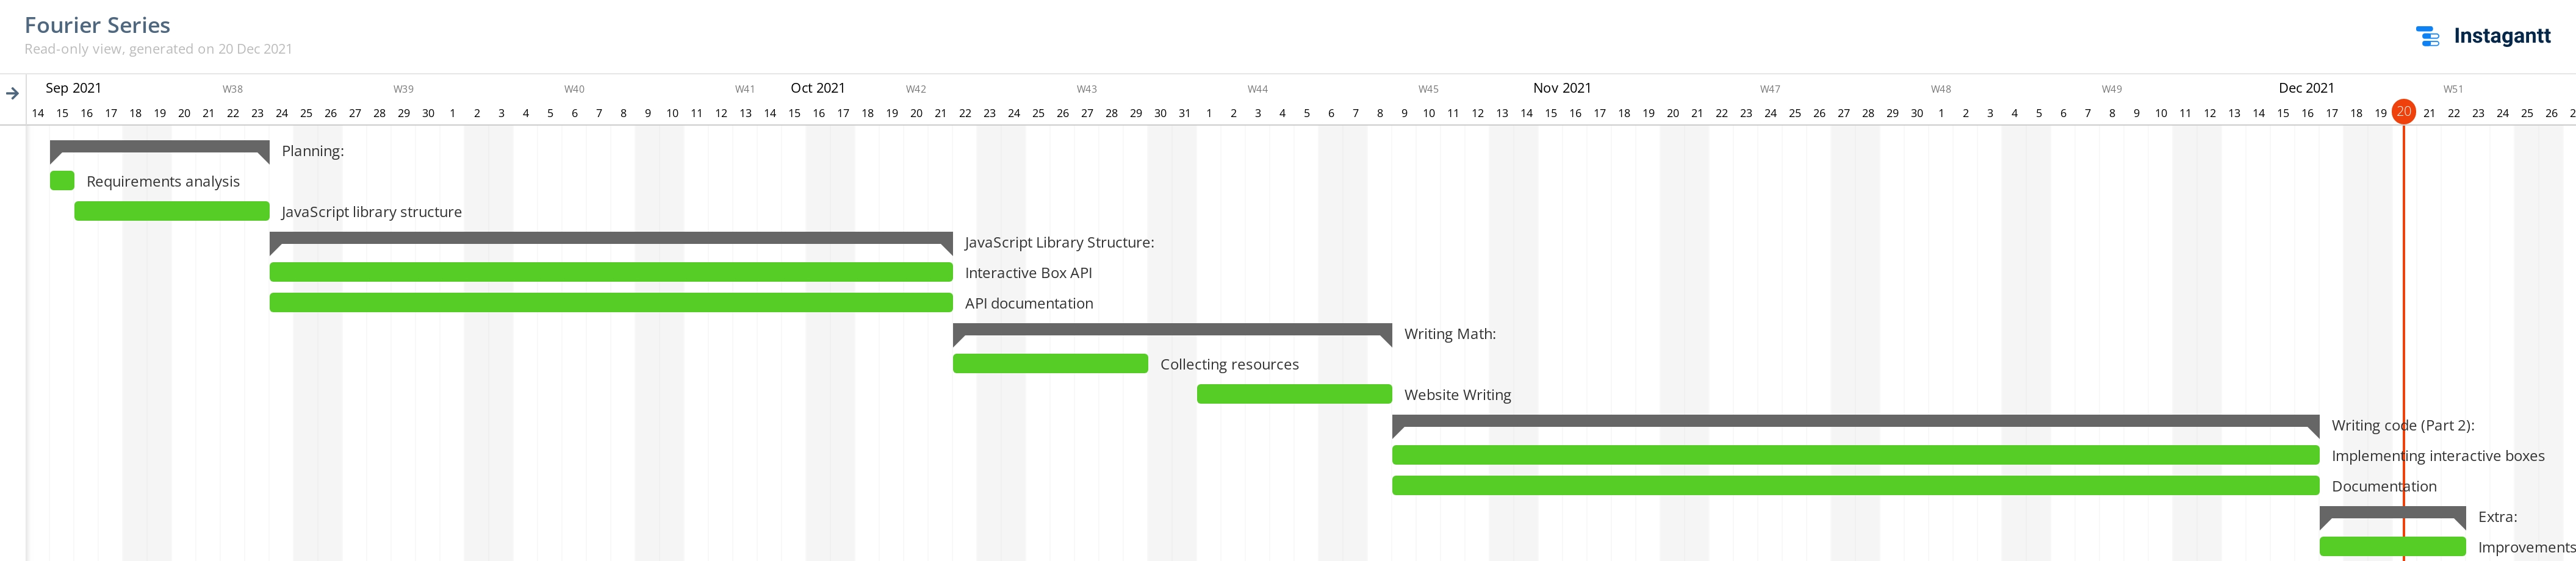
\includegraphics[width=\textwidth]{gantt1}

\subsubsection{Final Gantt Chart}

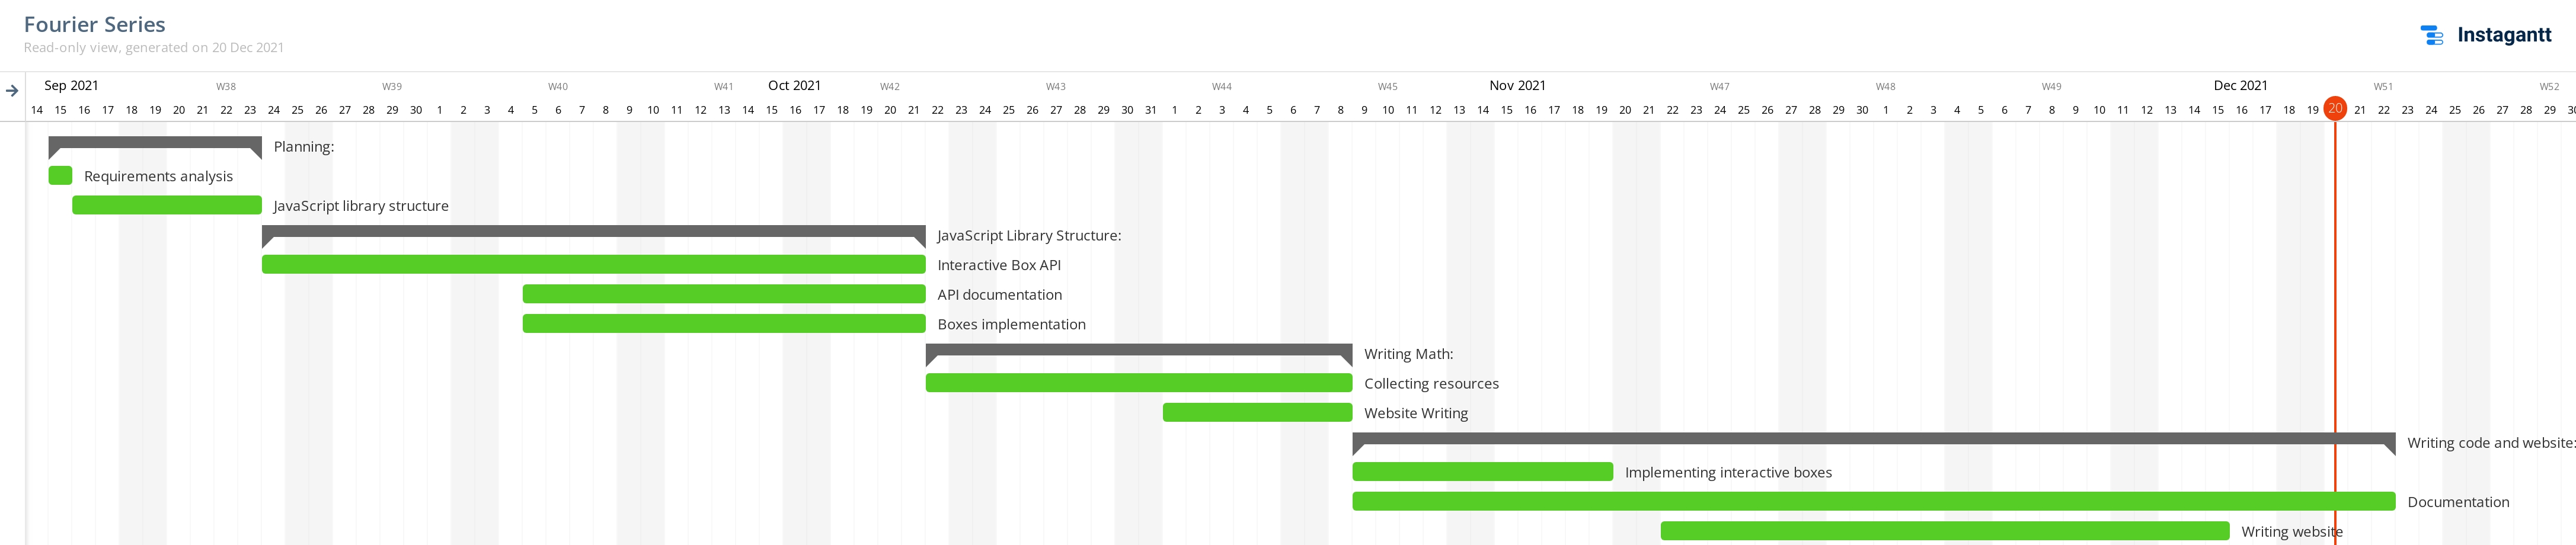
\includegraphics[width=\textwidth]{gantt2}

The various phases have been roughly respected, although I would sometimes work on some unscheduled tasks.

\pagebreak

\section{Interactive Boxes}

\subsection{Description}

InteractiveBoxes is a JavaScript library I wrote for canvas rendering based on the user input.
The library injects its content into a HTML div element. The content consists of a canvas element,
a stop/resume button and a range slider (the timeline), additional content is injected by the
interactive box implementations.
The user can interact with the timeline, pause and resume the animation or modify the input by simply drawing onto the canvas.

\subsection{Implementation}

To create an interactive box you need to create a class that extends \texttt{InteractiveBox.js}.
The class of your custom interactive box must override some functions, otherwise you will get errors.
You will also need to call the super constructor.
Here are the declaration of those function in the \texttt{InteractiveBox.js} class and its constructor.

\medskip

\begin{lstlisting}[style=js]
    constructor(name, container, height, width) {
        ...
    }

    draw(ctx) {
        throw 'The function draw() has not been overwritten'
    }

    setPoints(points) {
        throw 'The function setPoints(points) has not been overwritten'
    }

    onTimeTravel(value) {
        throw 'The function onTimeTravel(value) has not been overwritten'
    }
\end{lstlisting}

Overriding these functions will produce a class that looks like this

\begin{lstlisting}[style=js]

class MyCustomBox extends InteractiveBox {

    constructor(name, container, height, width) {
        super(name, container, height, width)

        // inject extra html, initialize variables, ...
    }

    draw(ctx) {
        this.clearCanvas();

        // draw function

        // update timeline
        this.setTime(...);
    }

    onTimeTravel(value) {
        // onTimeTravel function
    }

    setPoints(points) {
        // setPoints function
    }

}
\end{lstlisting}

\pagebreak

\subsection{List of Functions}

Here is a list of public functions in \texttt{InteractiveBox.js}

\bgroup{}
\def\arraystretch{1.5}
\begin{center}
    \begin{tabular}{ |l|l|l|l|}
        \hline
        \textbf{Name} & \textbf{Description} & \textbf{Parameters} & \textbf{Returns} \\
        \hline
        constructor() & Constructor &
        \makecell[l]{
            \tabitem \textbf{name} the name of the box \\
            \tabitem \textbf{container} the div id \\
            \tabitem \textbf{height} the height of the canvas \\
            \tabitem \textbf{width} the width of the canvas
        } & void \\
        \hline
        pause() & Pauses the animation & none & void \\
        \hline
        resume() & Resumes the animation & none & void \\
        \hline
        toggle() & \makecell[l]{Pauses or resumes \\ the animation} & none & void \\
        \hline
        isPlaying() &
        \makecell[l]{
            Returns \texttt{true} if \\
            the animation is playing
        } & none & bool \\
        \hline
        setTime() &
        \makecell[l]{
            Updates the timeline, \\
            you should call this in \\
            the draw() function}
        & \tabitem \textbf{value} the time value \(\in [0;1]\) & void \\
        \hline
        clearCanvas() & Clears the canvas & none & void \\
        \hline
        draw() &
        \makecell[l]{
            Called for each frame \\
            \textbf{Must override!}
        } & \tabitem \textbf{ctx} The canvas context & void \\
        \hline
        onTimeTravel() &
        \makecell[l]{
            Called when the user \\
            moves the timeline \\
            \textbf{Must override!}
        } & \tabitem \textbf{value} the time value \(\in [0;1]\) & void \\
        \hline
        setPoints() &
        \makecell[l]{
            Called when the user \\
            draws a path \\
            \textbf{Must override!}
        } & \tabitem \textbf{points} array of \texttt{\{x,y\}} & void \\
        \hline
    \end{tabular}
\end{center}
\egroup{}

\subsection{Injecting}

To inject the interactive box into the site we must create a div element to contain it.

\begin{lstlisting}[style=html]
    <body>
        <!-- Here I place my MyCustomBox-->
        <div id="mycustombox-div">
        </div>
    </body>
\end{lstlisting}

Then, in a JavaScript environment add the box to the div

\begin{lstlisting}[style=js]
    new MyCustomBox('mycustombox1', 'mycustombox-div-box', 500, 500);
\end{lstlisting}

In order for everything to work you must include the \texttt{InteractiveBox.js} file, your \texttt{MyCustomBox.js}
file and the InteractiveBoxes css stylesheet \texttt{boxes.css}.

Note: the name must be unique, and the script must be executed after the body has loaded.

\pagebreak

\subsection{Example}

Here is an example of interactive box where the path drawn by the user is progressively drawn on the canvas.

\begin{lstlisting}[style=js]
    class Example extends InteractiveBox {

        #points = []; // The path to be drawn
        #counter = 0; // Drawing progress

        constructor(name, container, height, width) {
            super(name, container, height, width)

            this.setPoints(this.#getDefaultPath());
        }

        onTimeTravel(value) {
            // Set counter accoring to value
            this.#counter = value * this.#points.length | 0;
        }

        setPoints(points) {
            this.#counter = 0; // Reset counter
            this.#points = points; // Update points
        };

        draw(ctx) {
            this.clearCanvas(); // Clear the canvas
            
            // Update counter and update timeline
            this.setTime(this.#counter++ / (this.#points.length - 1));
            if (this.#counter > this.#points.length) {
                this.#counter = 0; // Reset counter
            }

            ctx.beginPath();
            
            ctx.lineWidth = 2.0;
            ctx.strokeStyle = 'red';

            ctx.moveTo(this.#points[0].x, this.#points[0].y);
            for (var i = 1; i < this.#counter; i++) {
                ctx.lineTo(this.#points[i].x, this.#points[i].y);
            }

            ctx.stroke();
        };

        #getDefaultPath() {
            var circle = [];
            for (var i = 0; i < 100; i++) {
                circle[i] = {
                    x: 250 + 50 * Math.cos(Math.PI * 2 / 100 * i),
                    y: 250 + 50 * Math.sin(Math.PI * 2 / 100 * i)
                }
            }
            return circle;
        }

    }
\end{lstlisting}

\pagebreak

\section{Website Implementation}

\subsection{Dependency table}

The website relies on various libraries, some of which are not stored locally.
This means that the user will query third-party servers, thus the website will not work
locally if you do not have a free internet connection.

\medskip

\bgroup{}
\def\arraystretch{1.5}
\begin{center}
    \begin{tabular}{ |p{3cm}|p{4cm}|p{2cm}|p{2cm}| }
        \hline
        \multicolumn{4}{|c|}{\textbf{Dependency table}} \\
        \hline
        \textbf{Name} & \textbf{Description} & \textbf{Stored} & \textbf{Version} \\
        \hline
        Bootstrap (CSS) & Styling framework & Locally & 4.0.0 \\
        \hline
        Bootstrap (JS) & Styling framework & Locally & 4.0.0 \\
        \hline
        InteractiveBoxes & Canvas drawing & Locally & 1.0 \\
        \hline
        JQuery & Website Manipulation & Locally & 3.6.0 \\
        \hline
        Google Fonts & Fonts & Remotely & - \\
        \hline
        MathJax & LaTeX rendering & Remotely & 3.x.x (latest) \\
        \hline
        Desmos & Graphing calculator & Remotely & 1.6 \\
        \hline
    \end{tabular}
\end{center}
\egroup{}

\pagebreak

\subsection{Sections}

The website is made up of several sections, each about a particular topic.

\subsubsection{Fourier Analysis}

What is Fourier analysis and where is it used.

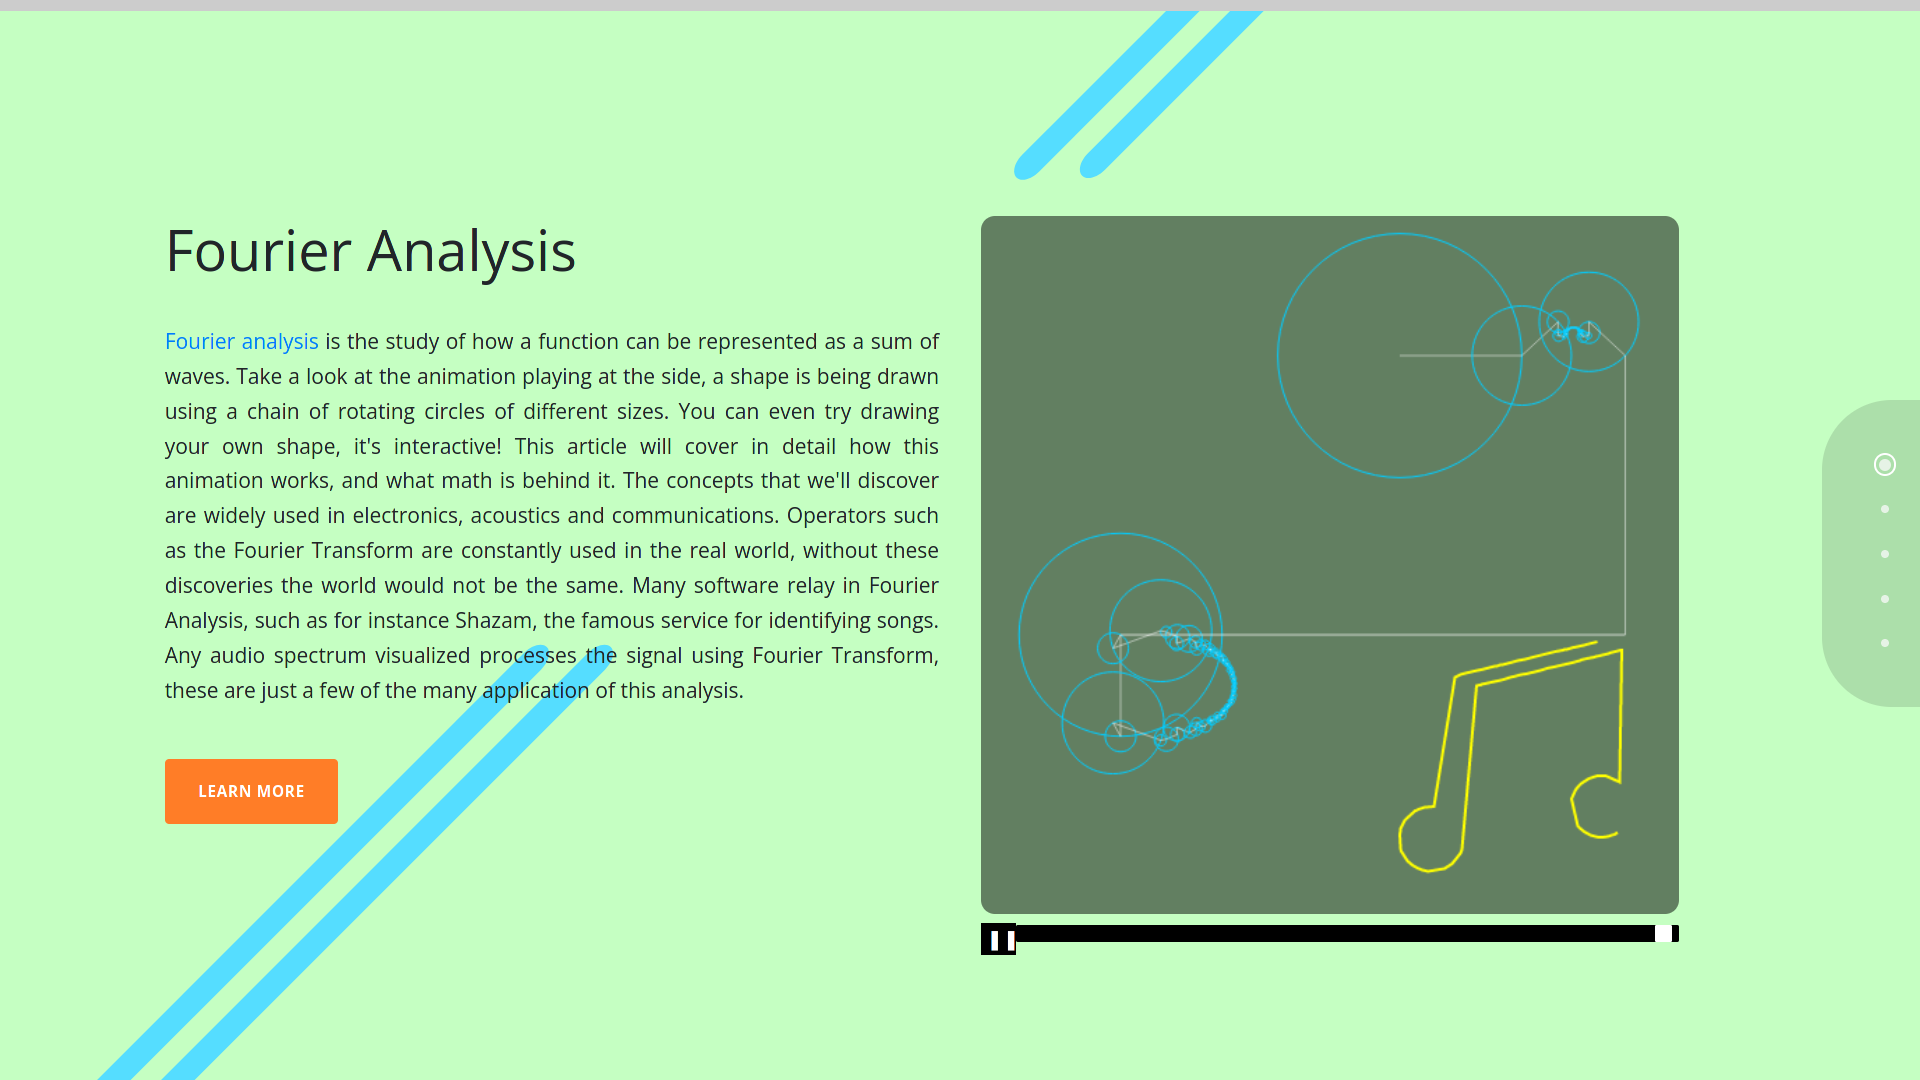
\includegraphics[width=\textwidth]{chap1.png}

\pagebreak

\subsubsection{Requirements}

What are the requirements to read the article.

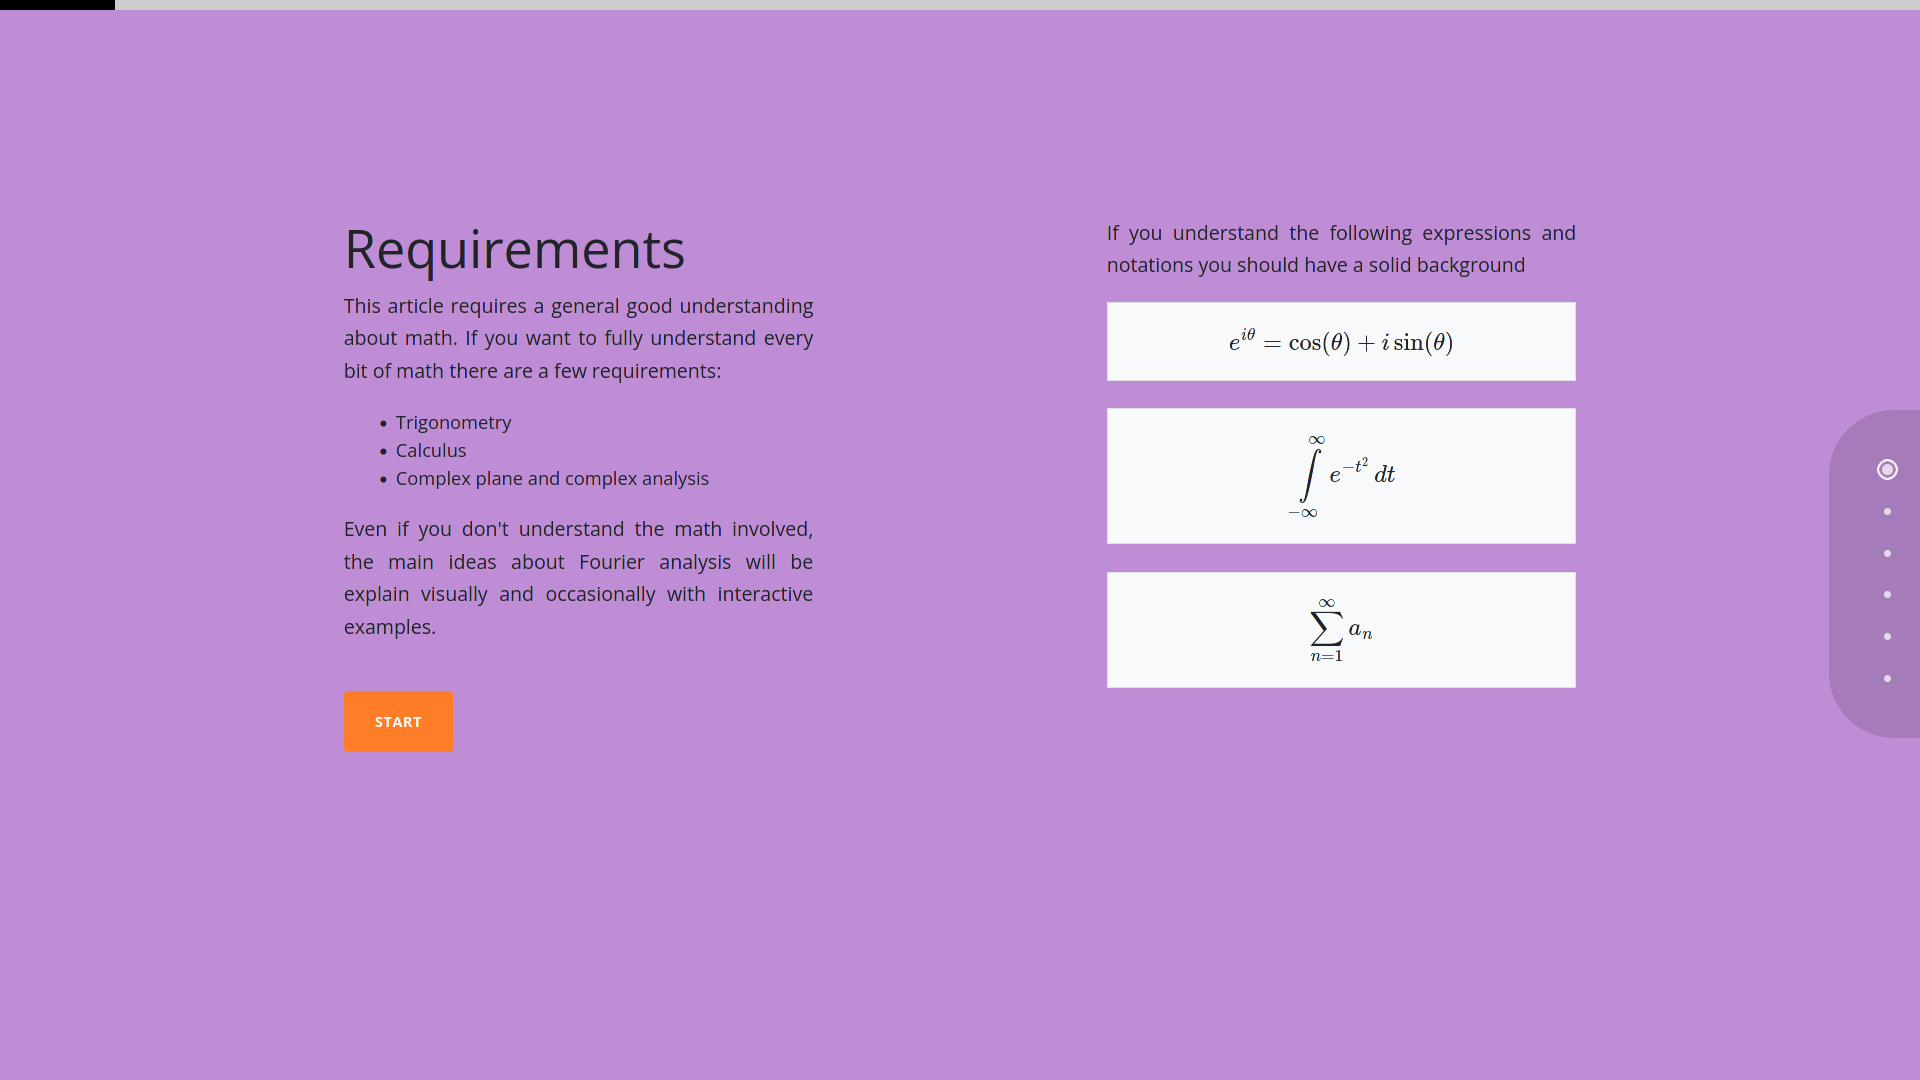
\includegraphics[width=\textwidth]{chap2.png}

\subsubsection{Introduction}

Who was Joseph Fourier and what he had discovered.

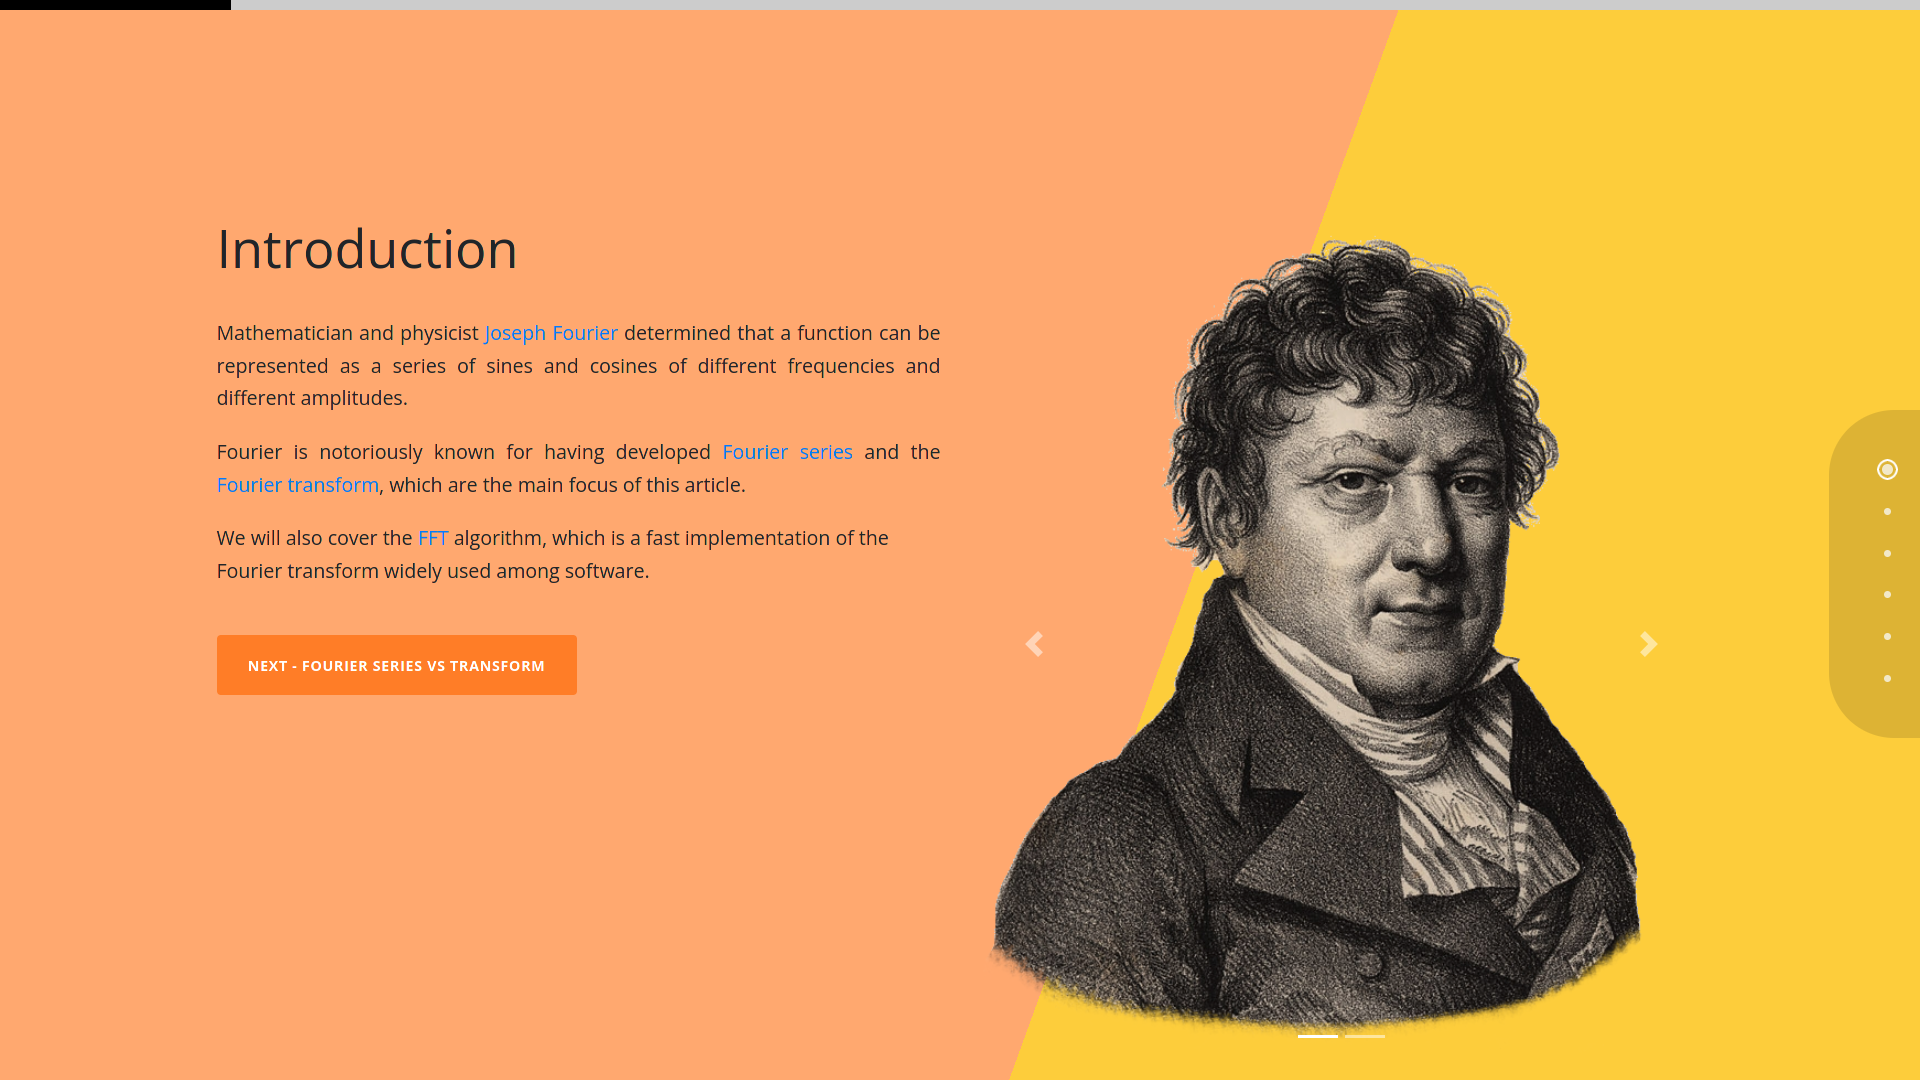
\includegraphics[width=\textwidth]{chap3.png}

\subsubsection{Fourier Series vs Fourier Transform}

What is the difference between the Furier series and the Fourier transform.

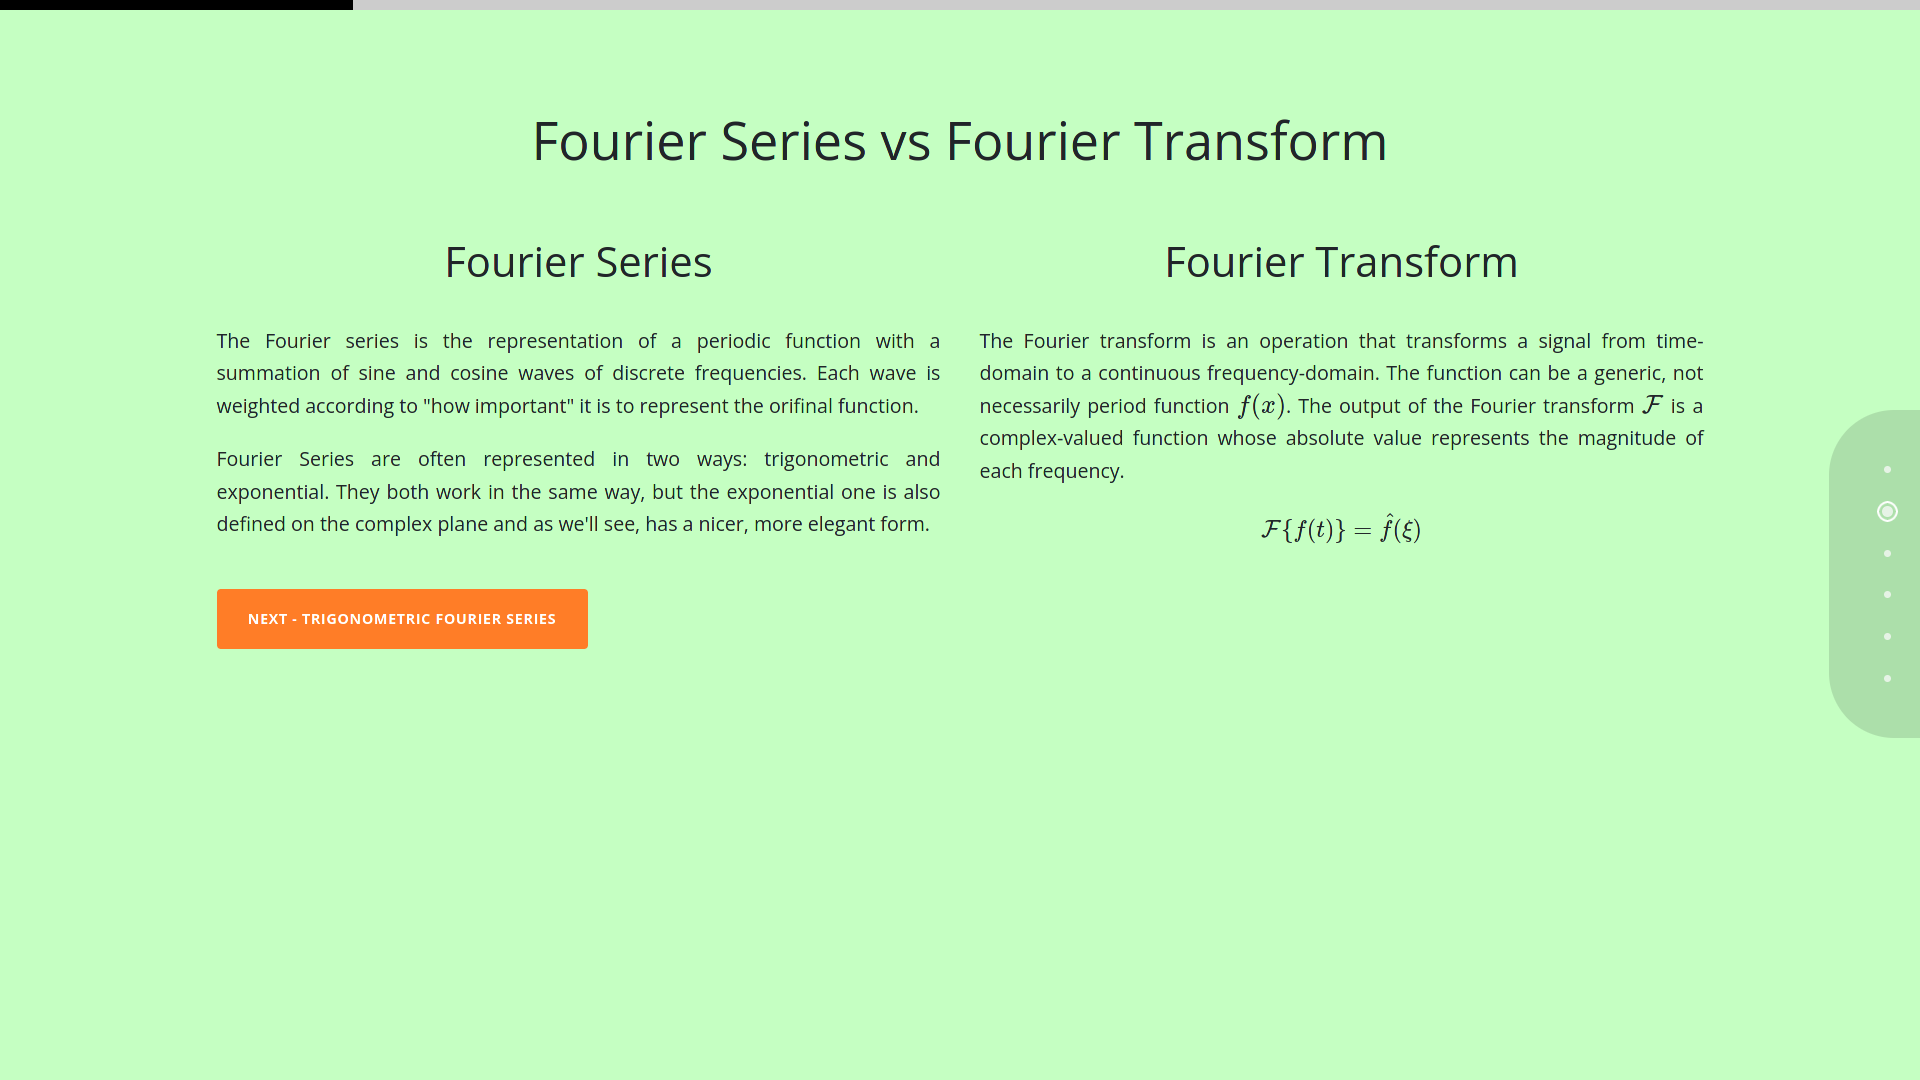
\includegraphics[width=\textwidth]{chap4.png}

\subsubsection{Trigonometric Fourier Series}

Representing a periodic function using a sum of trigonometric functions.

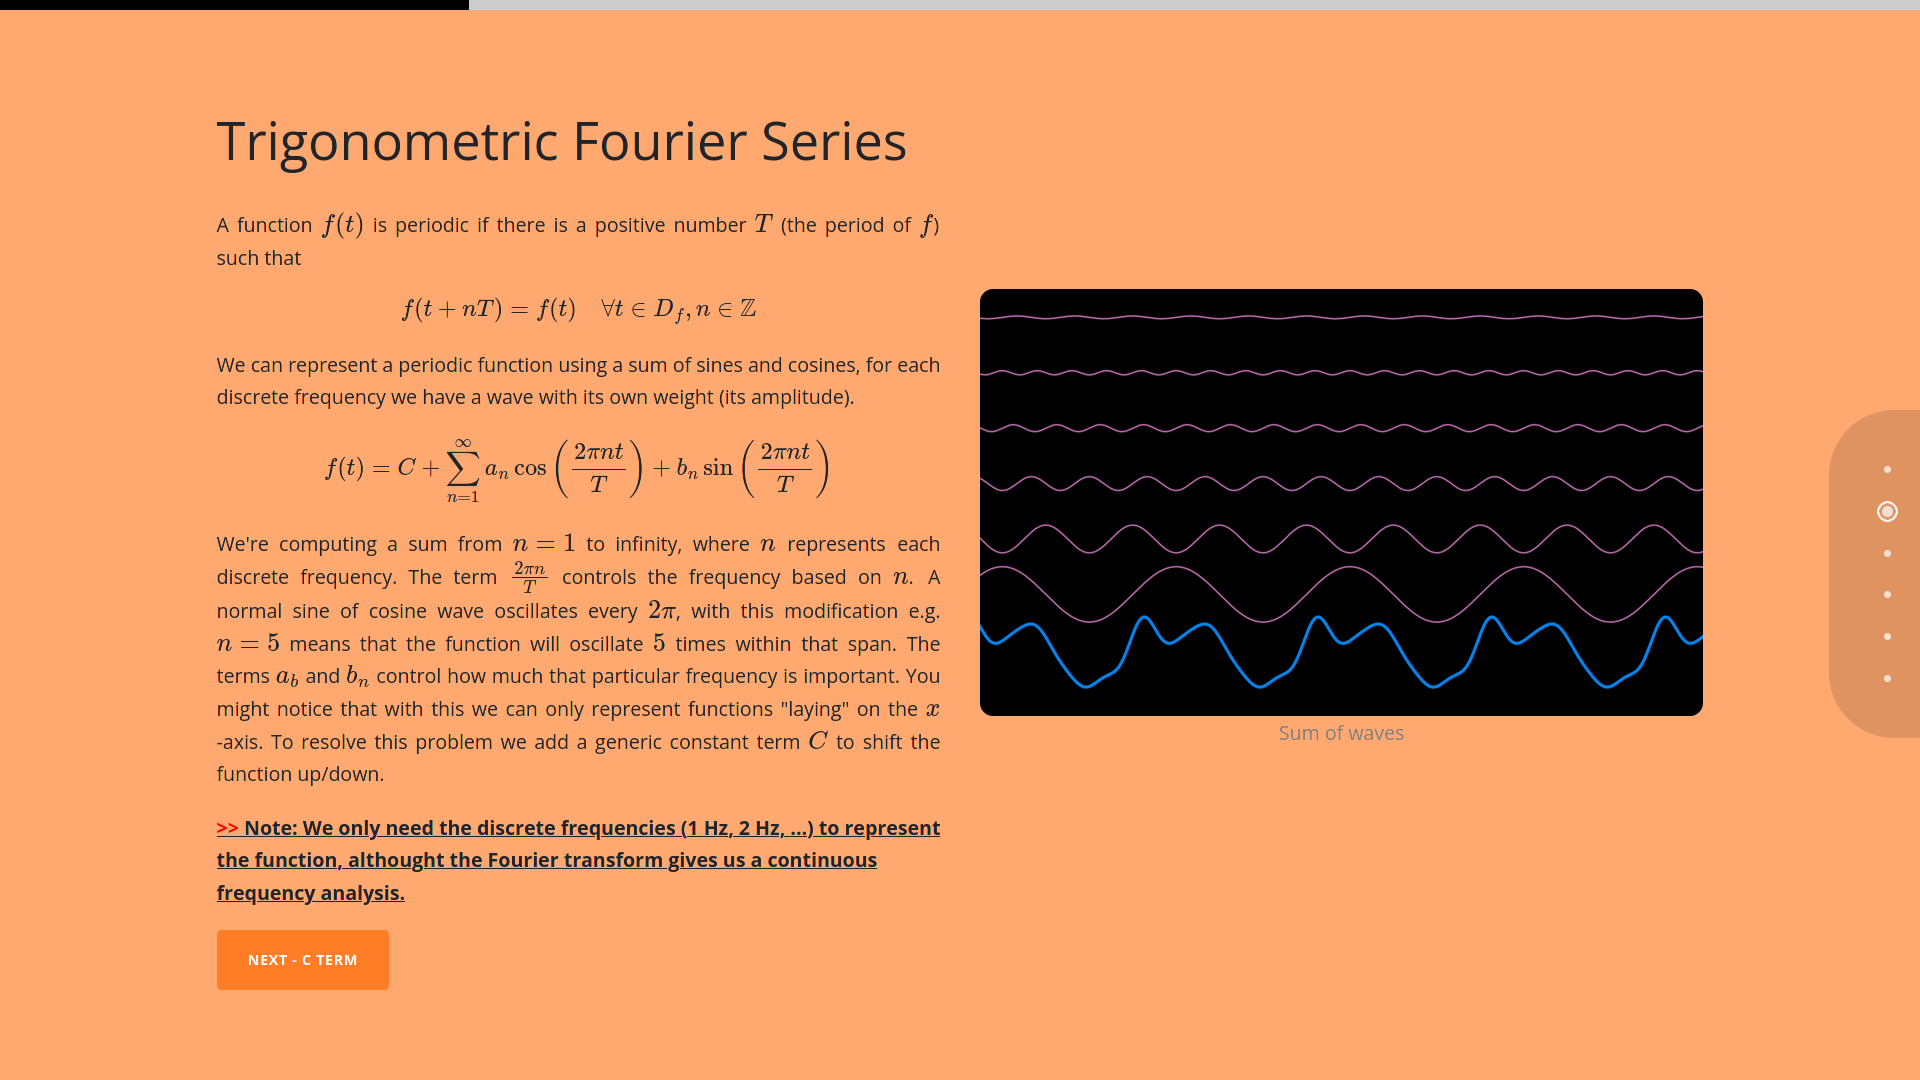
\includegraphics[width=\textwidth]{chap5.png}

\subsubsection{Trigonometric Fourier Series - C term}

Finding the \(C\) term.

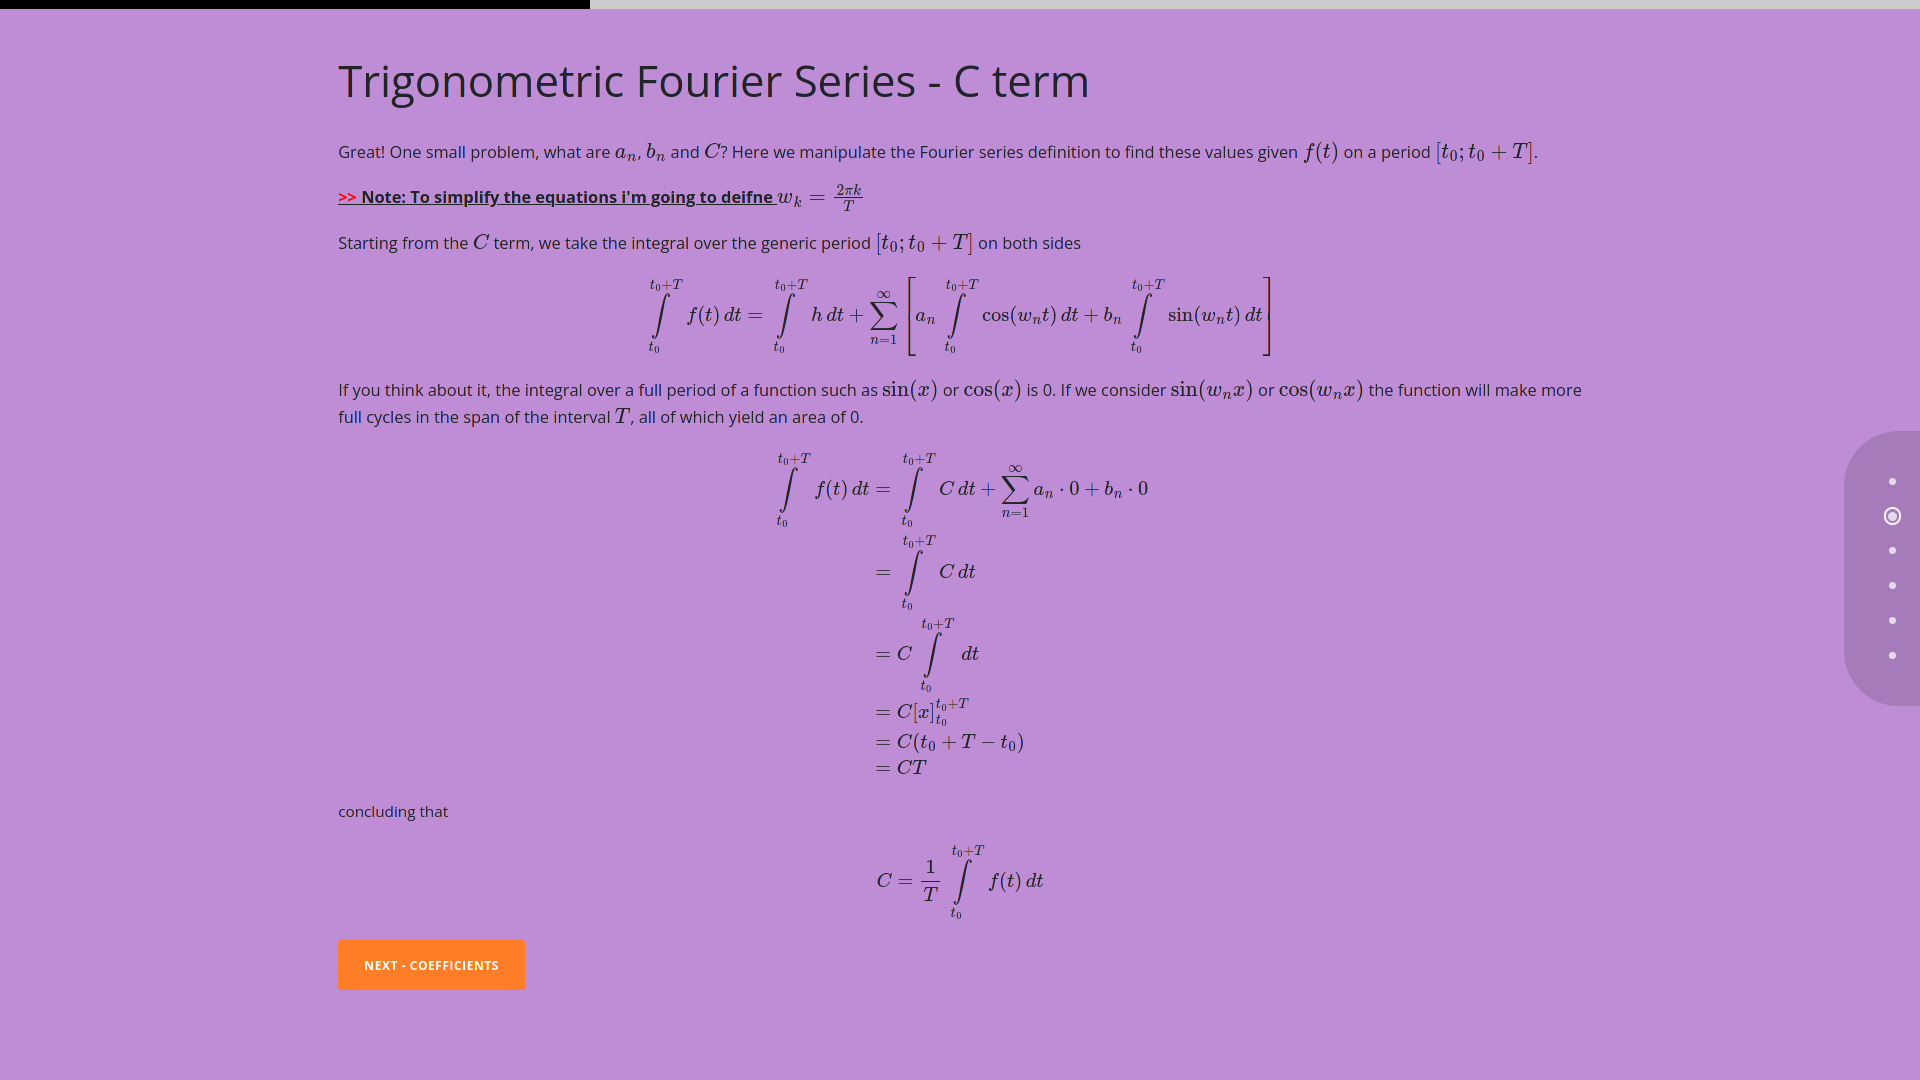
\includegraphics[width=\textwidth]{chap6.png}

\subsubsection{Trigonometric Fourier Series - Coefficients}

Finding the coefficients \(a_n\) and \(b_n\).

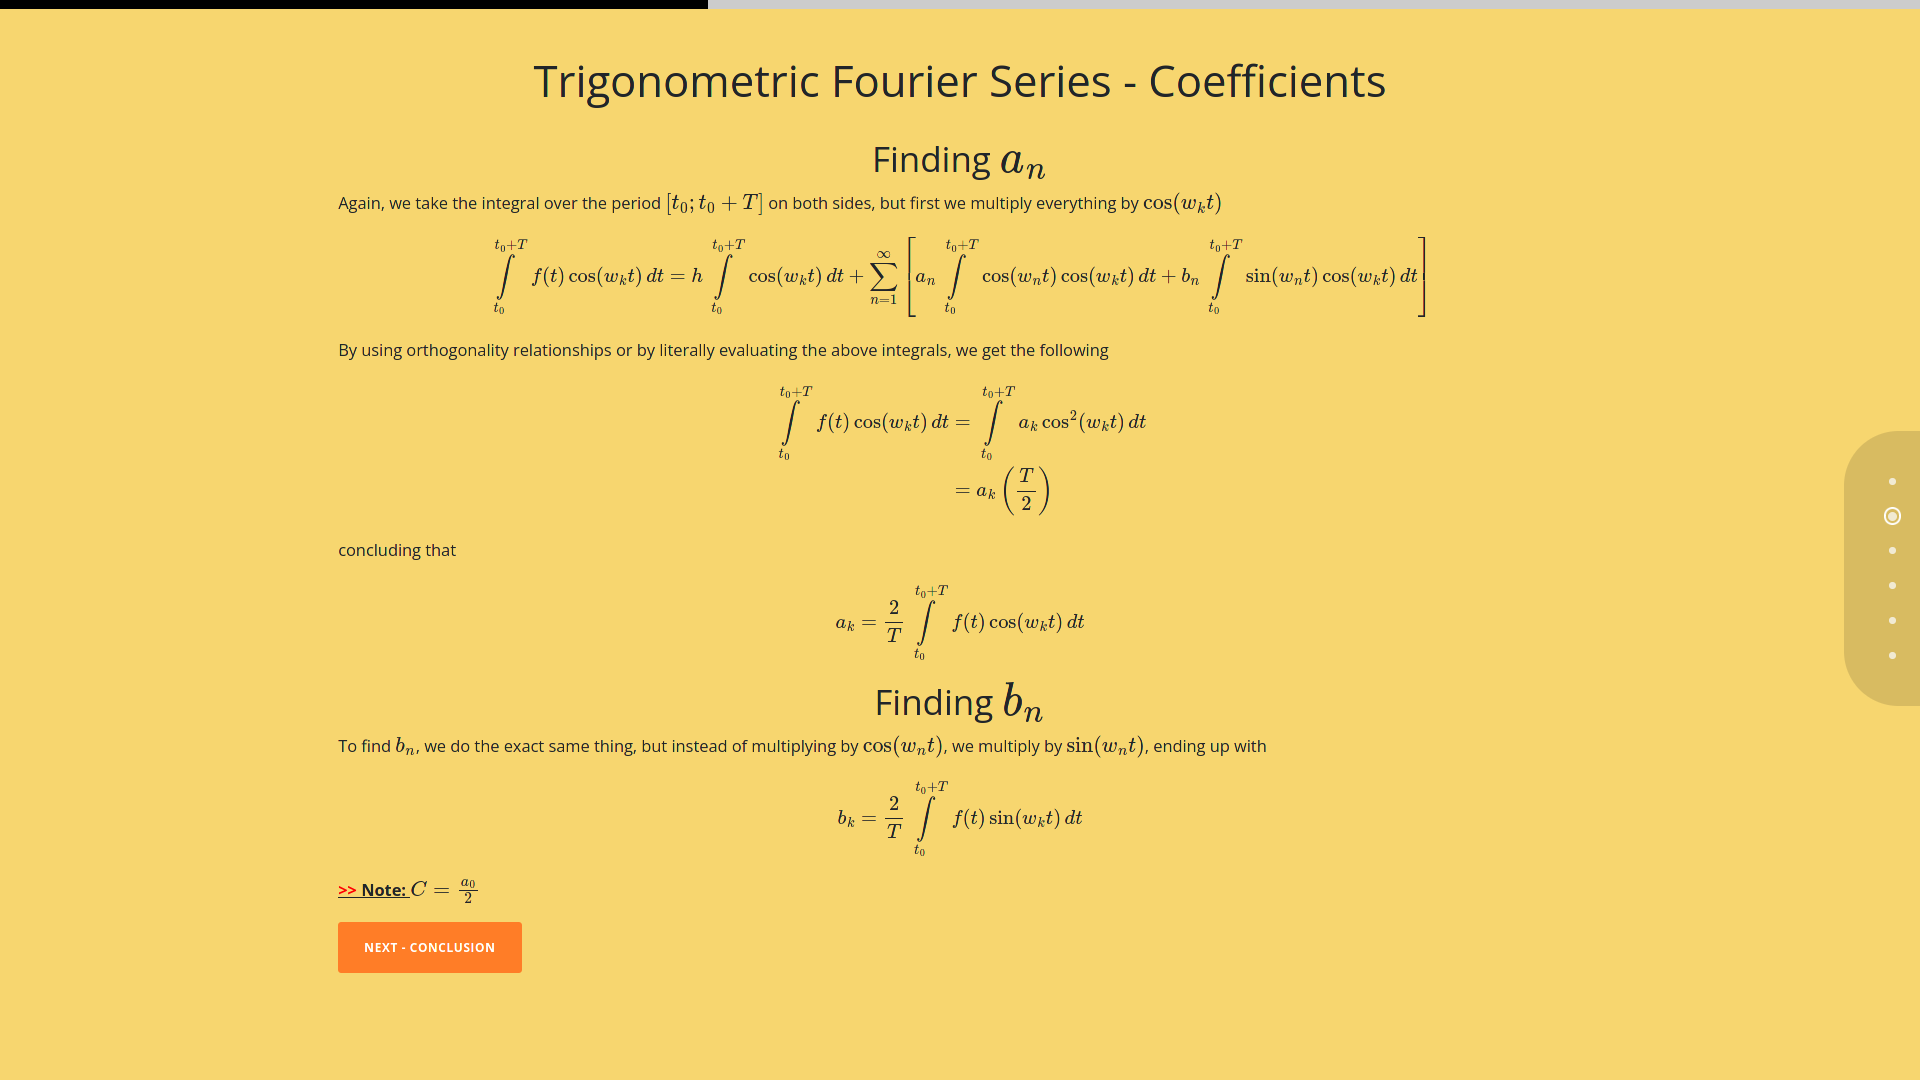
\includegraphics[width=\textwidth]{chap7.png}

\subsubsection{Fourier Series - Conclusion}

Conclusion on the last chapters.

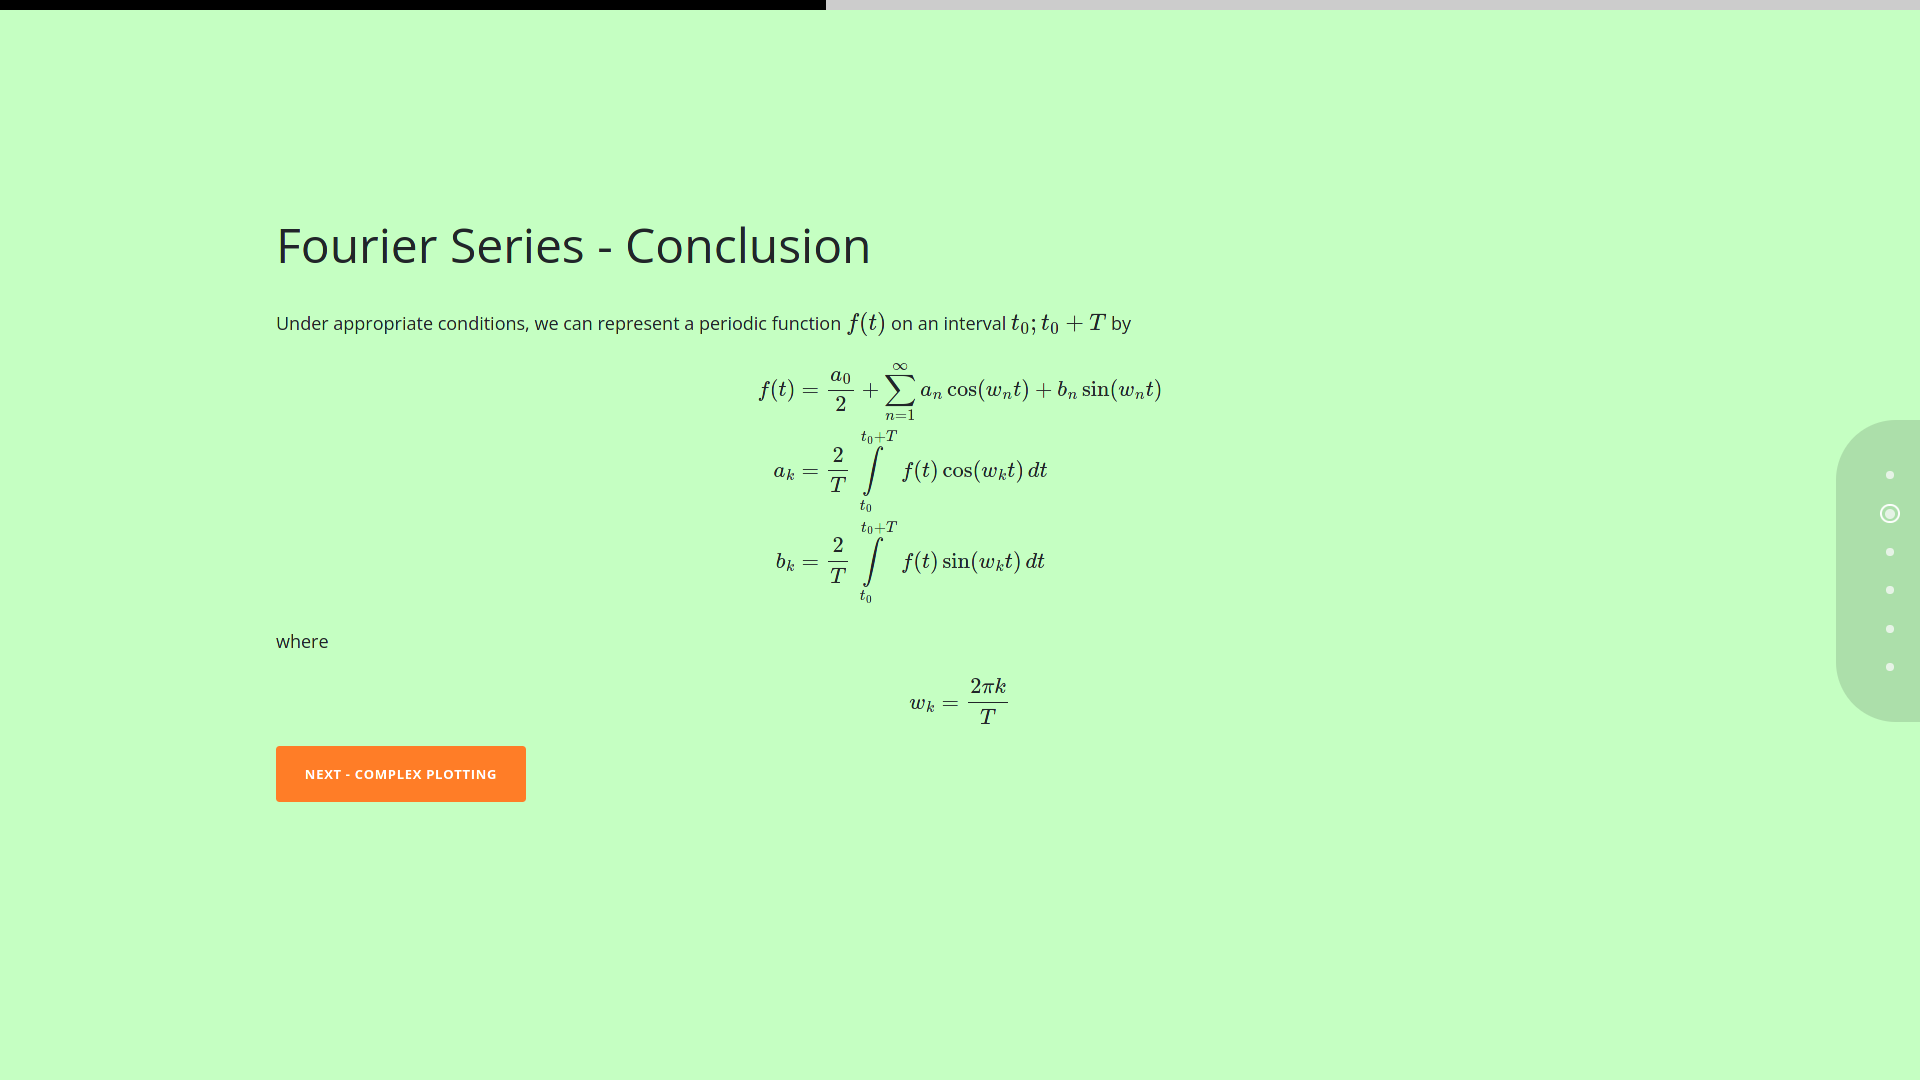
\includegraphics[width=\textwidth]{chap8.png}

\subsubsection{Main ideas - Complex plotting}

Plotting a function around the origin in the complex plane using Euler's identity.

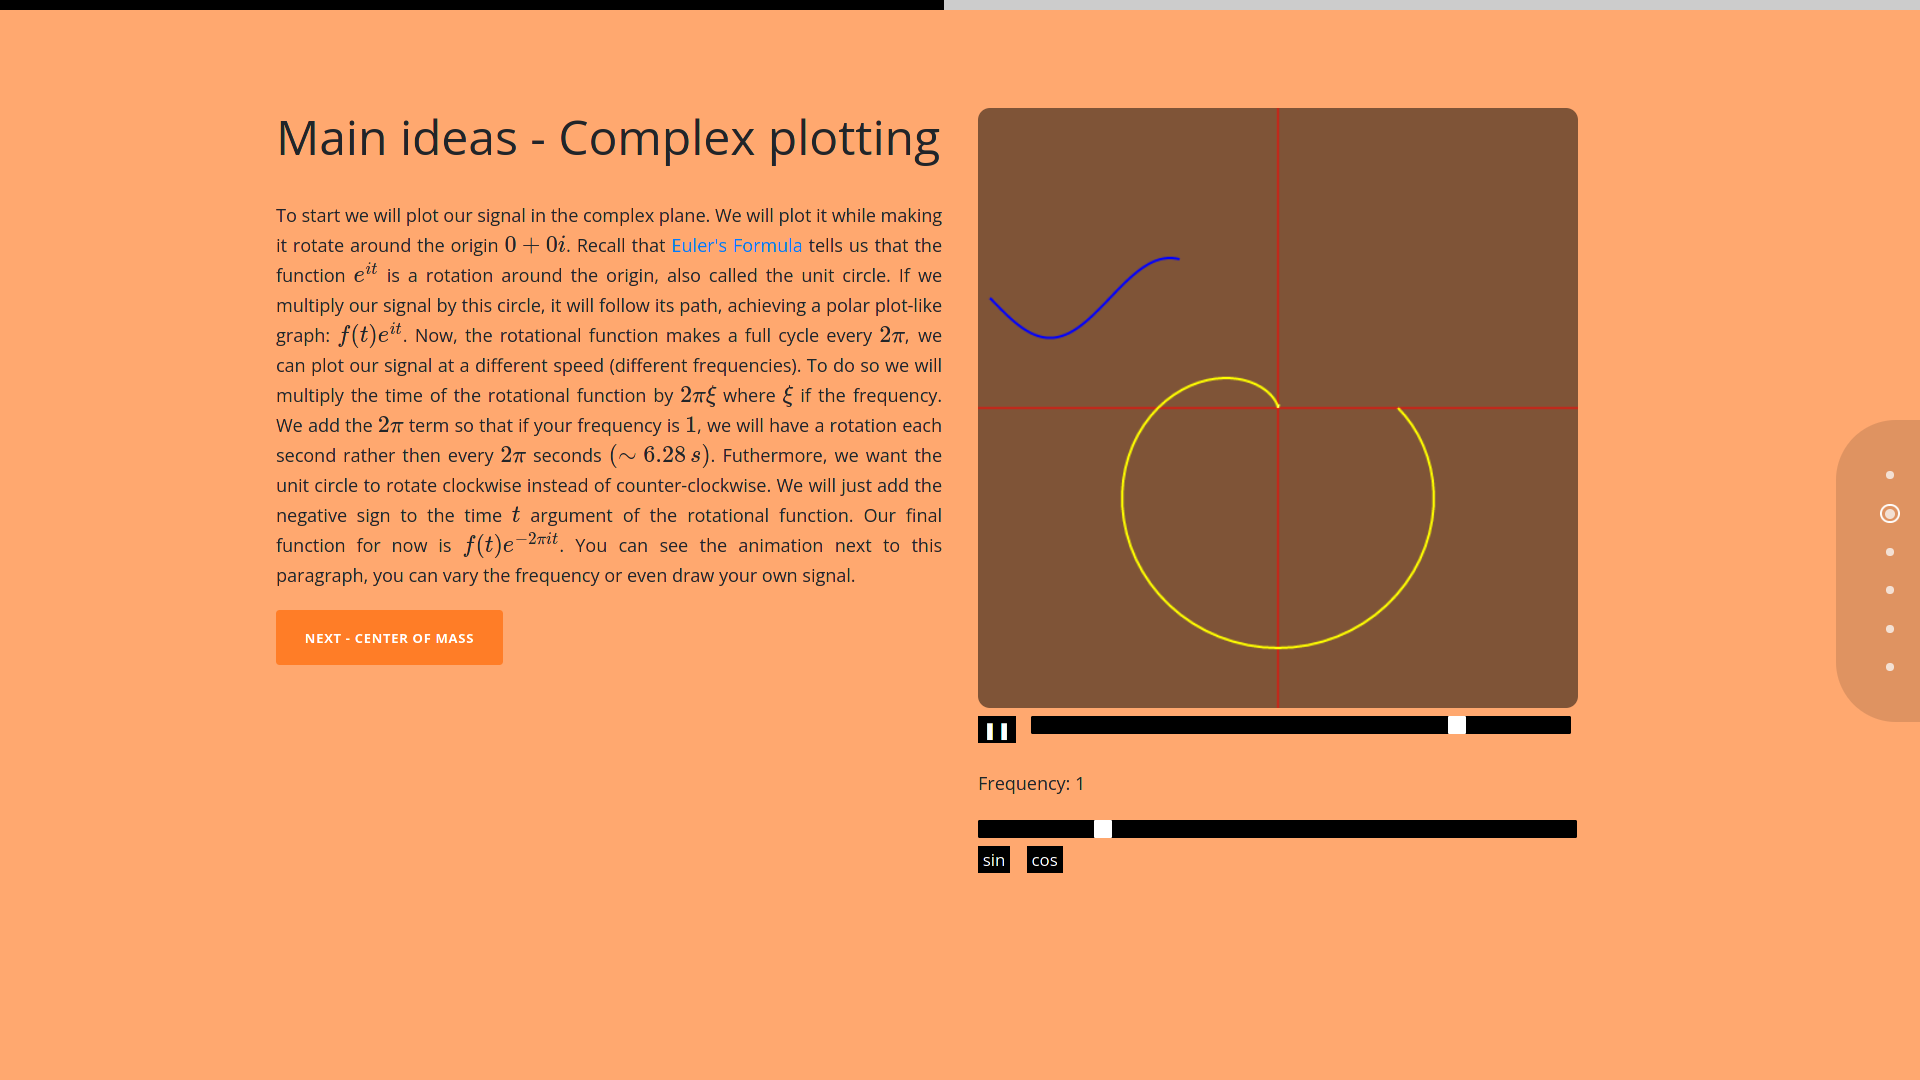
\includegraphics[width=\textwidth]{chap9.png}

\subsubsection{Main ideas - Center of mass}

Computing the center of mass of \(f(t)e^{-2\pi ti\xi}\)

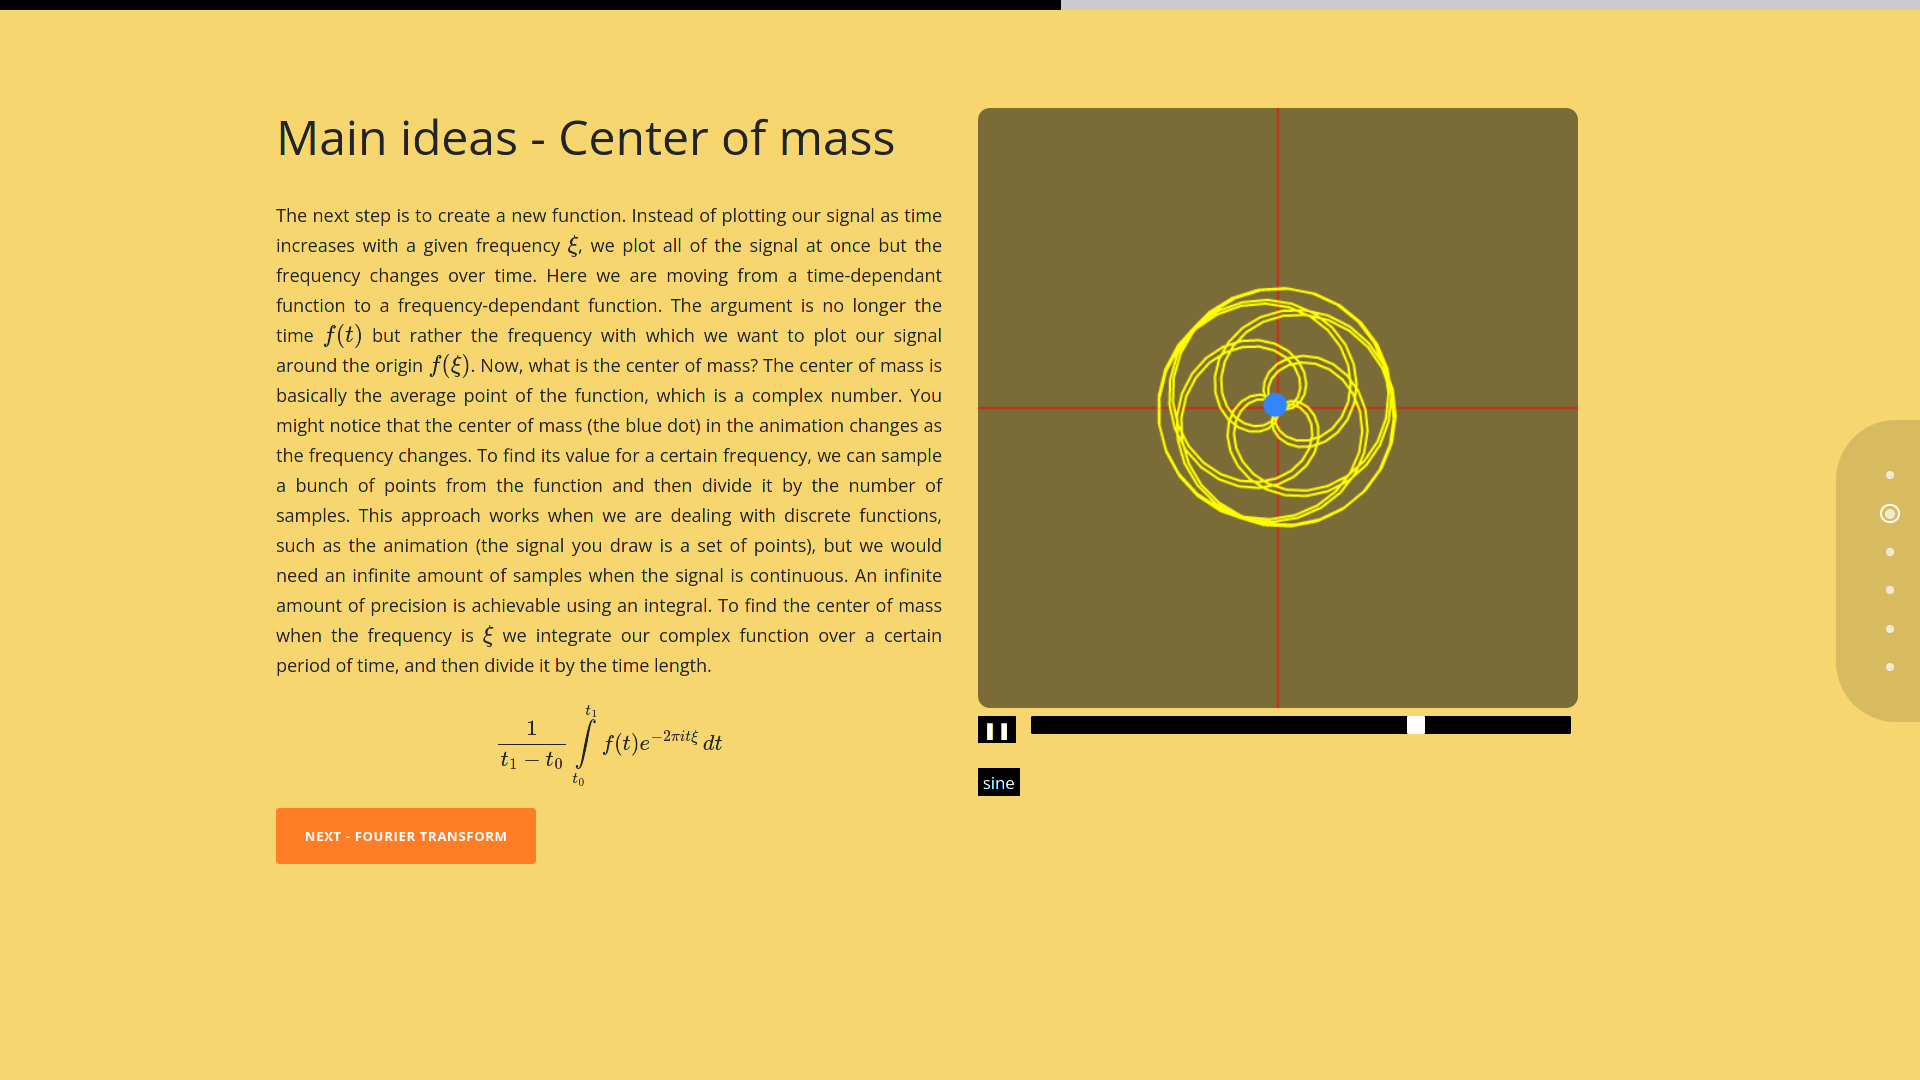
\includegraphics[width=\textwidth]{chap10.png}

\subsubsection{Main ideas - Fourier Transform}

What is the Fourier transform operator.

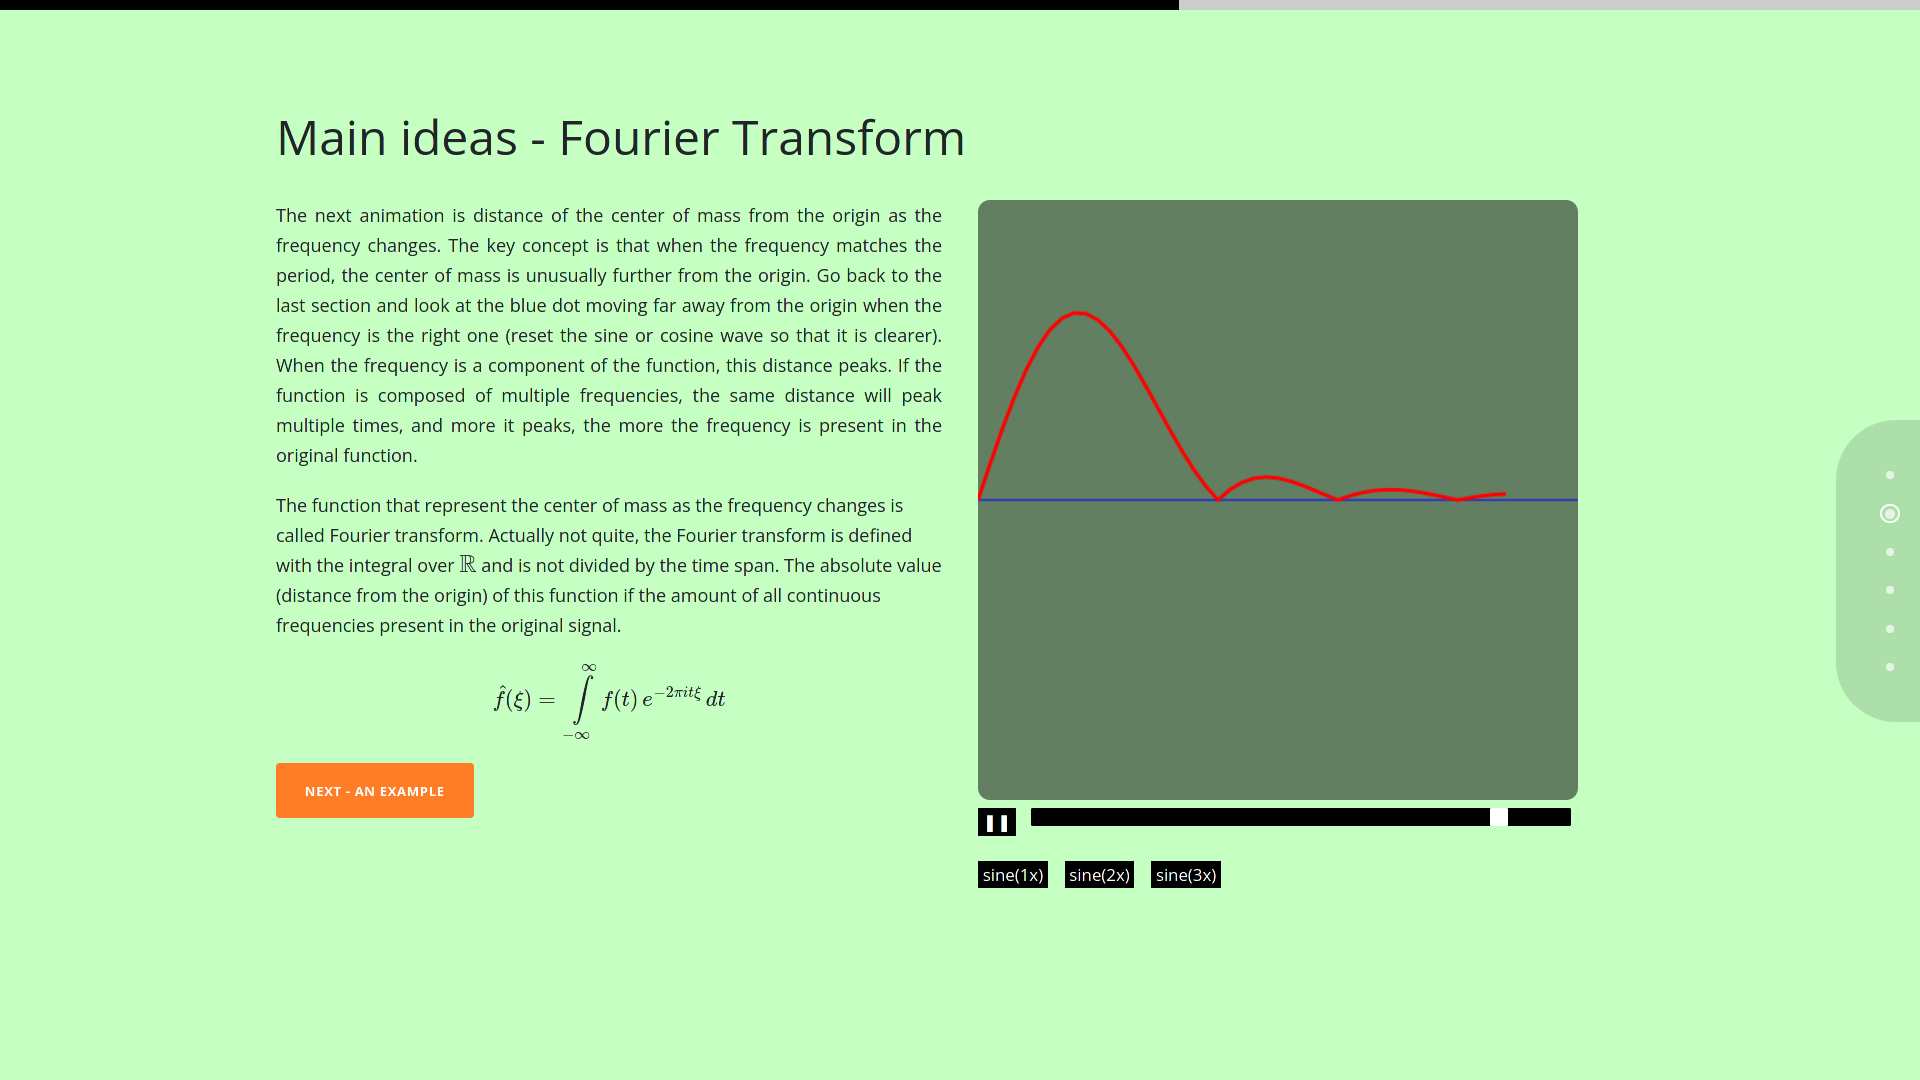
\includegraphics[width=\textwidth]{chap11.png}

\subsubsection{A Simple Example}

Computing the Fourier series of a simple function.

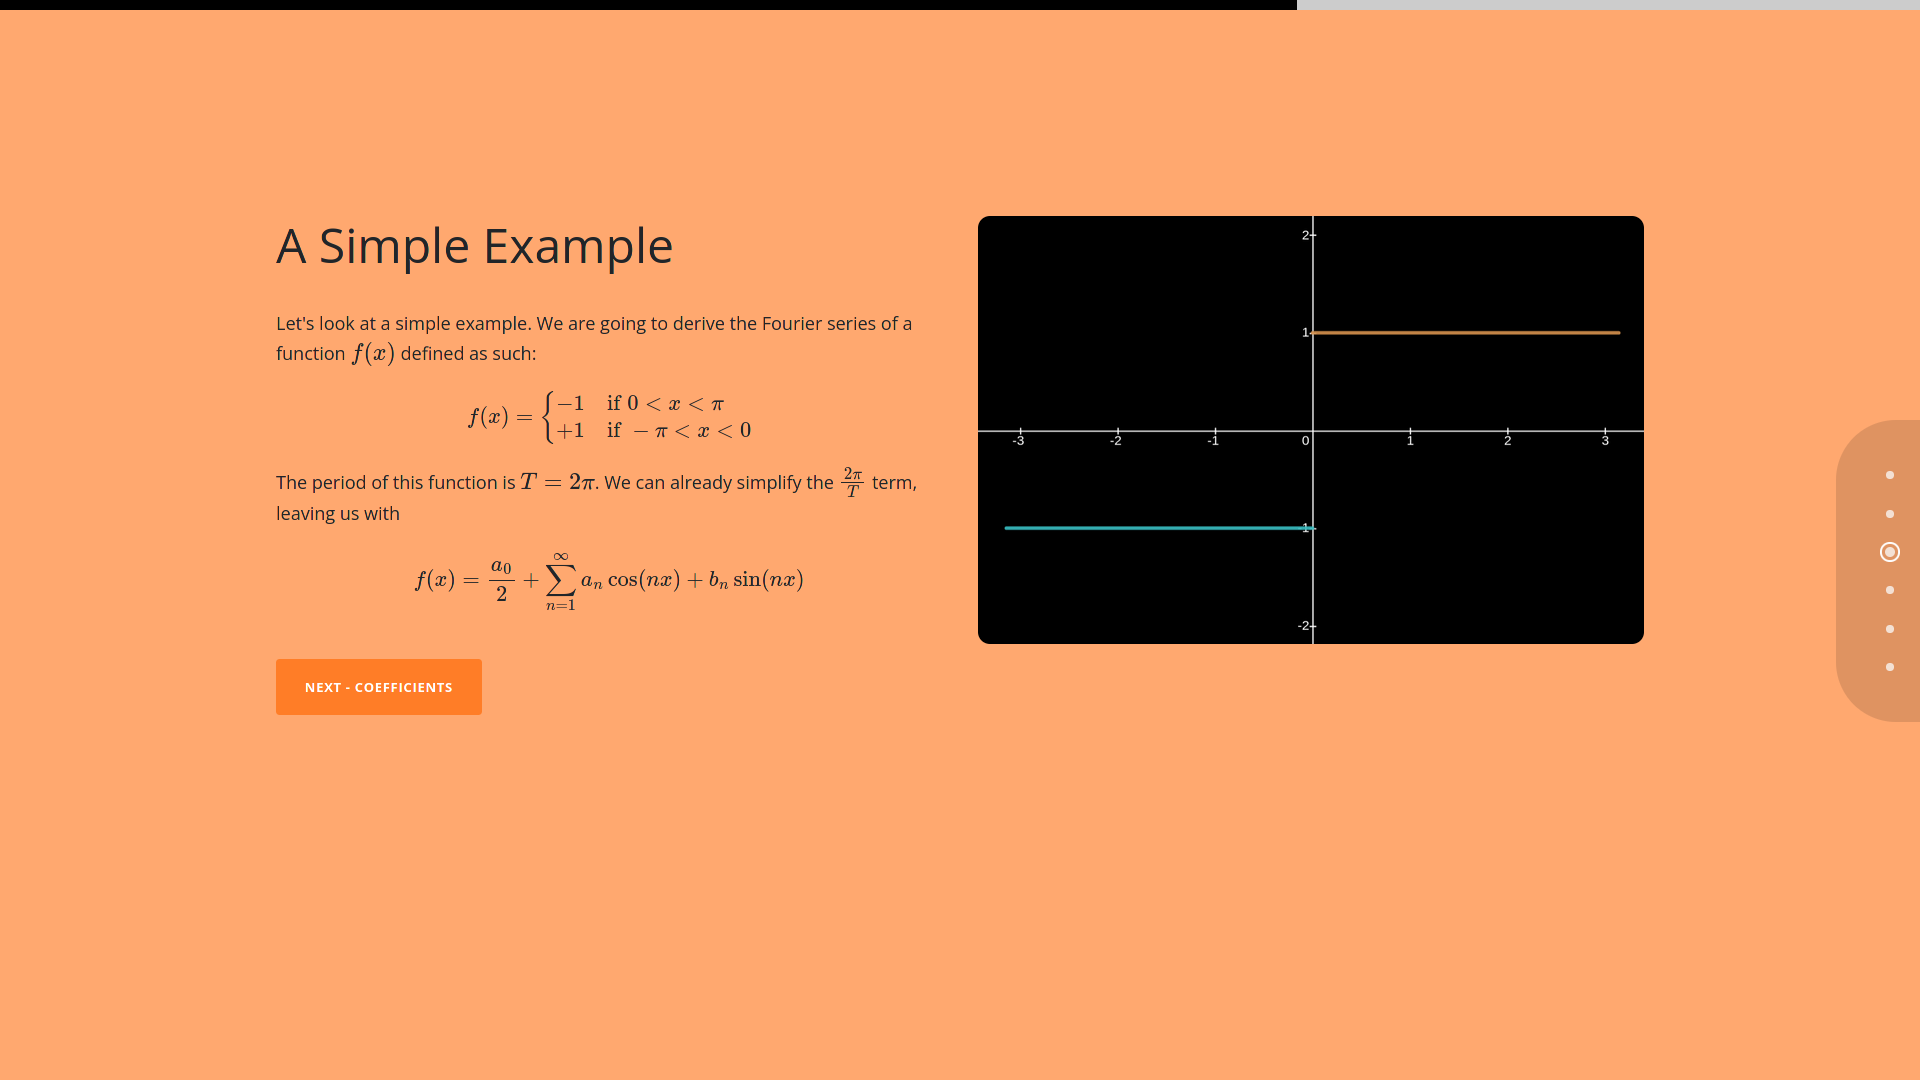
\includegraphics[width=\textwidth]{chap12.png}

\subsubsection{A Simple Example - Coefficients}

Finding the coefficients of the Fourier series.

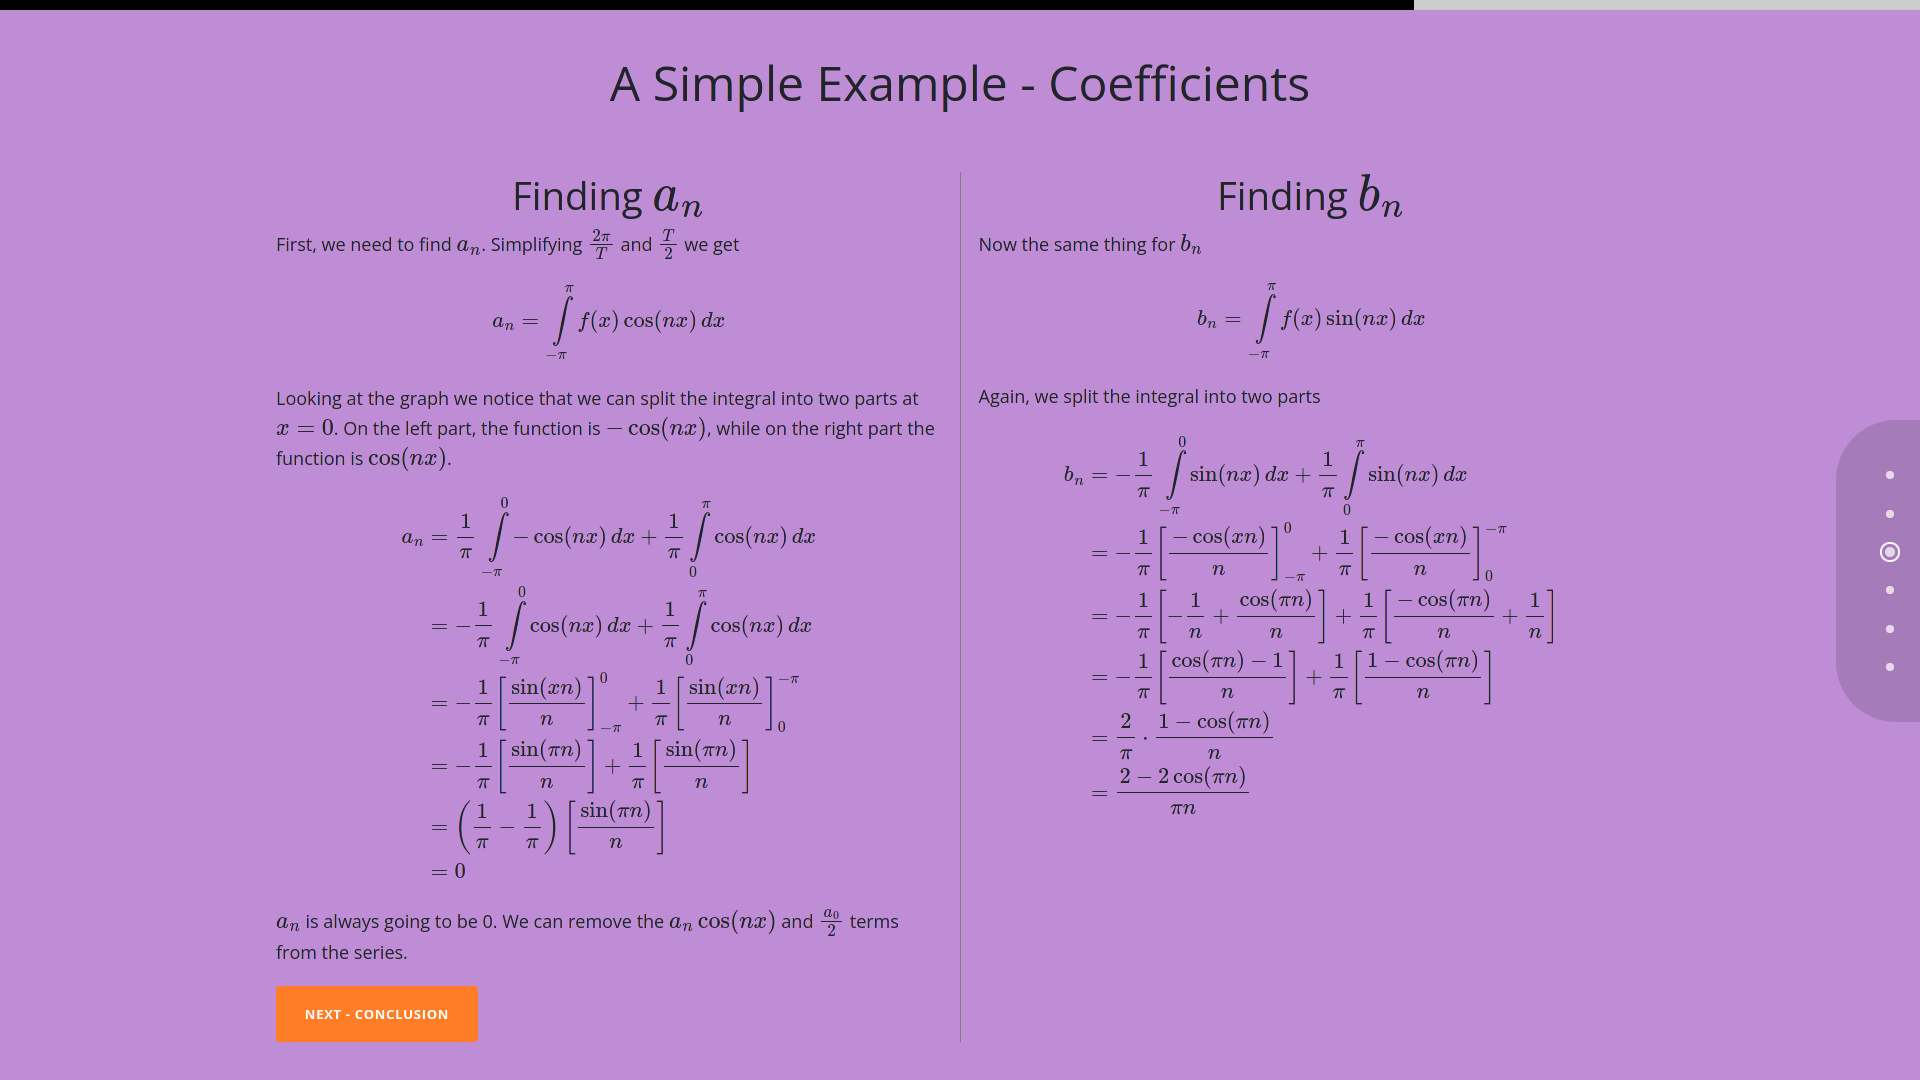
\includegraphics[width=\textwidth]{chap13.png}

\subsubsection{A Simple Example - Conclusion}

Demostrating the Fourier series by plotting it.

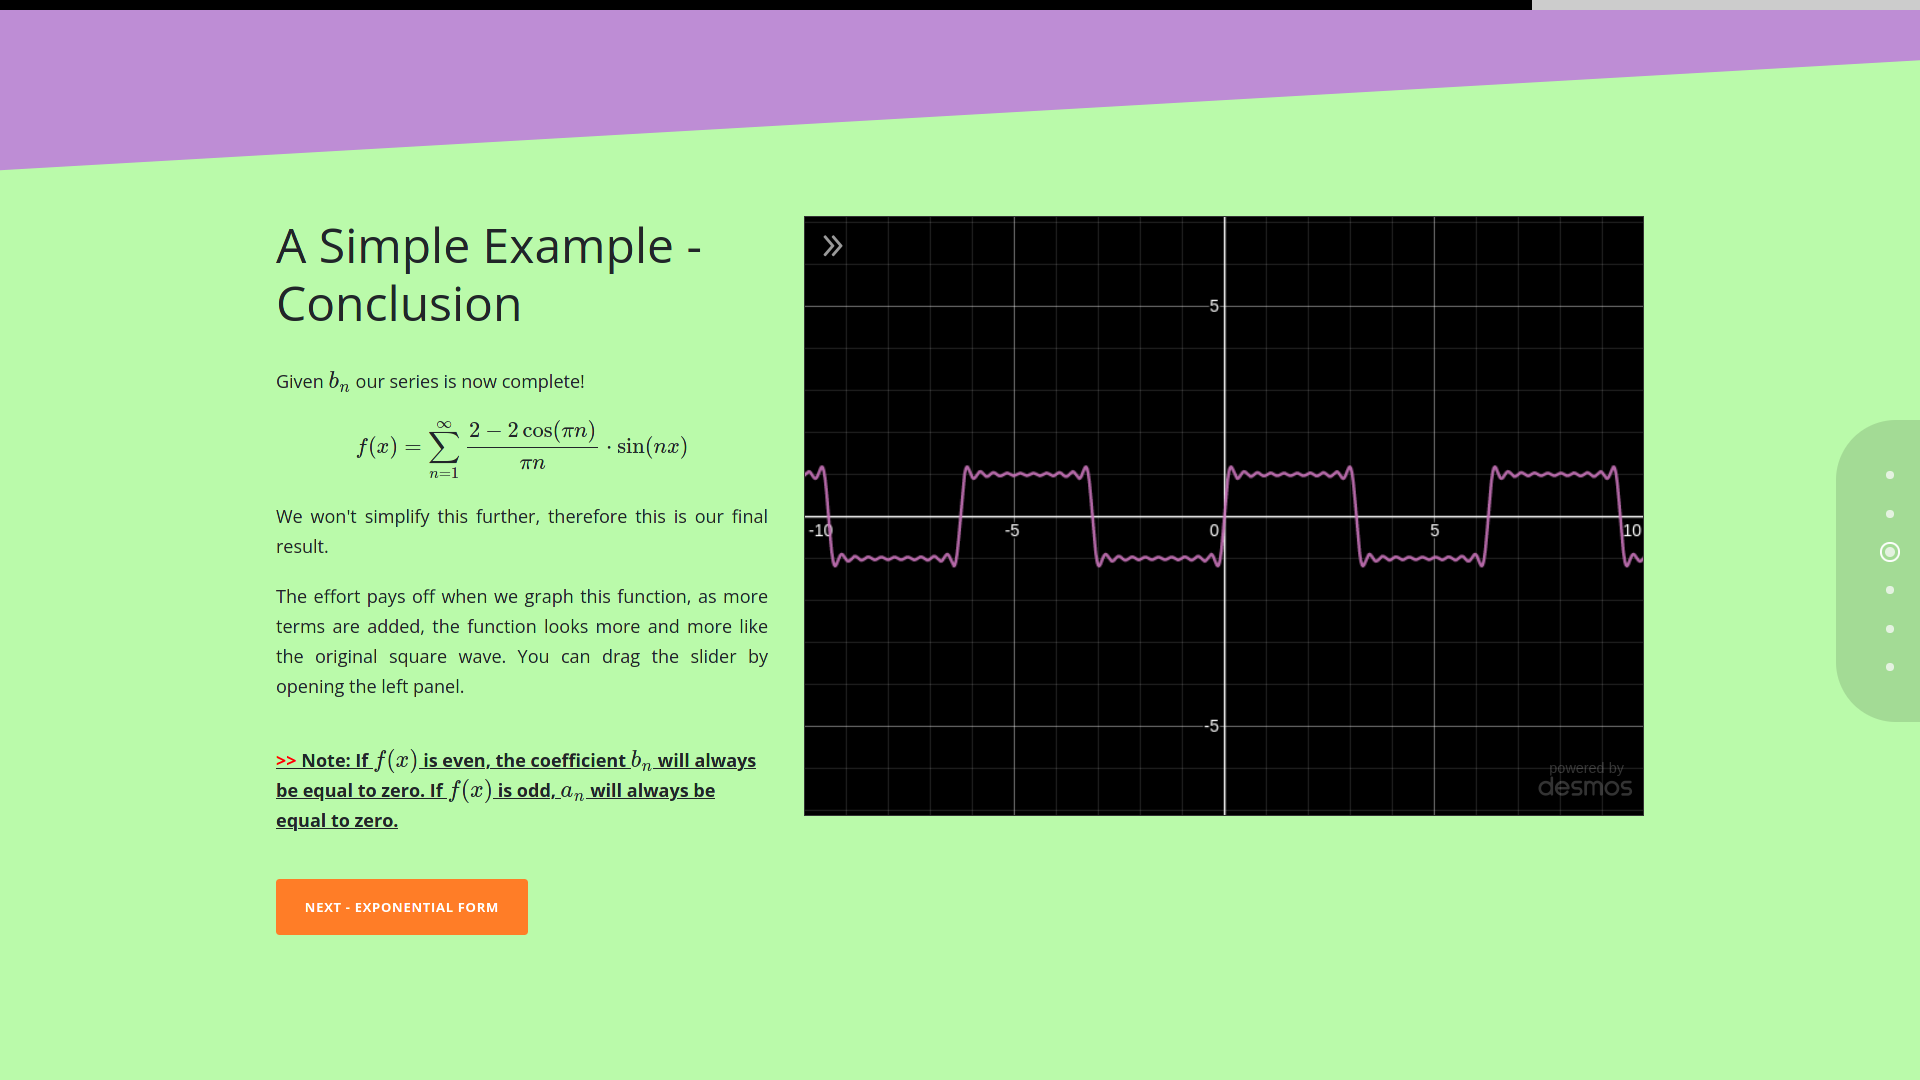
\includegraphics[width=\textwidth]{chap14.png}

\subsubsection{Exponential Fourier Series}

Defining the Fourier series using Euler's Identity.

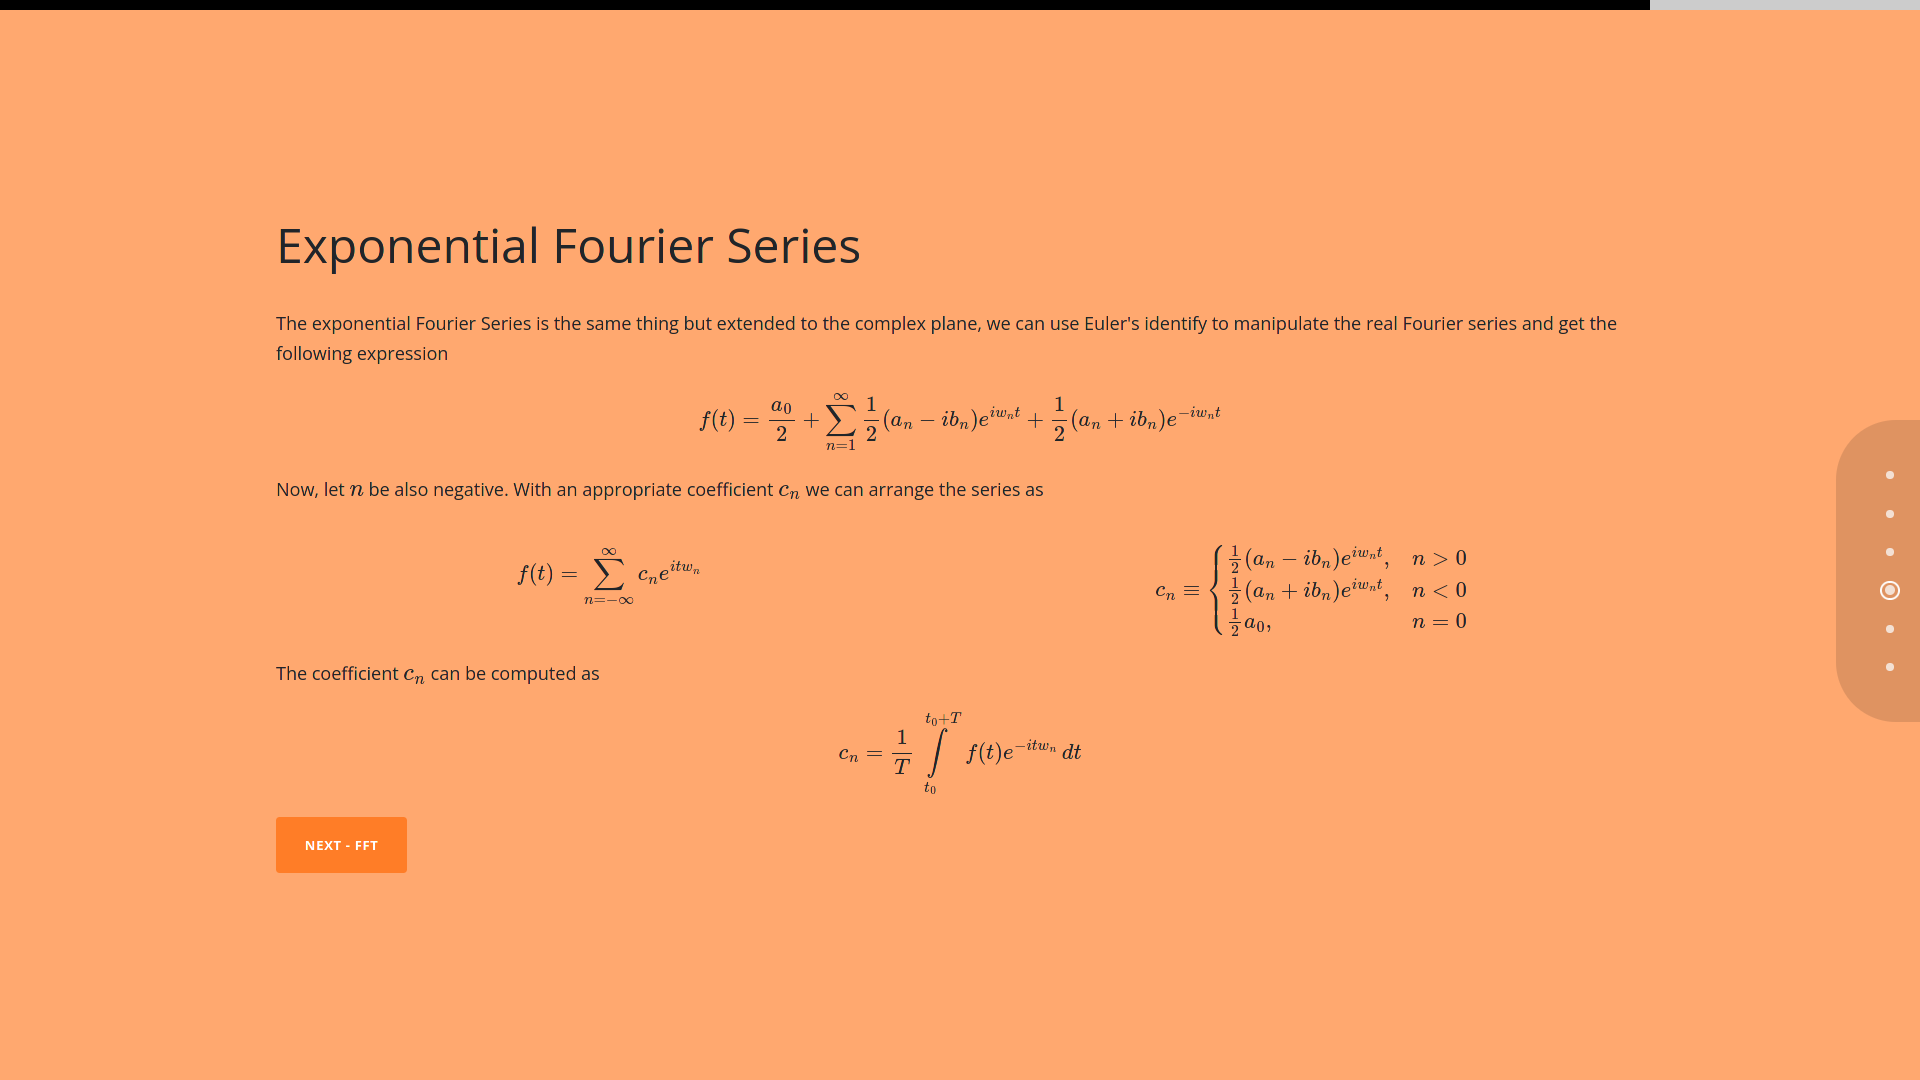
\includegraphics[width=\textwidth]{chap15.png}

\subsubsection{Fast Fourier Transform}

What is the Fast Fourier Transform algorithm.

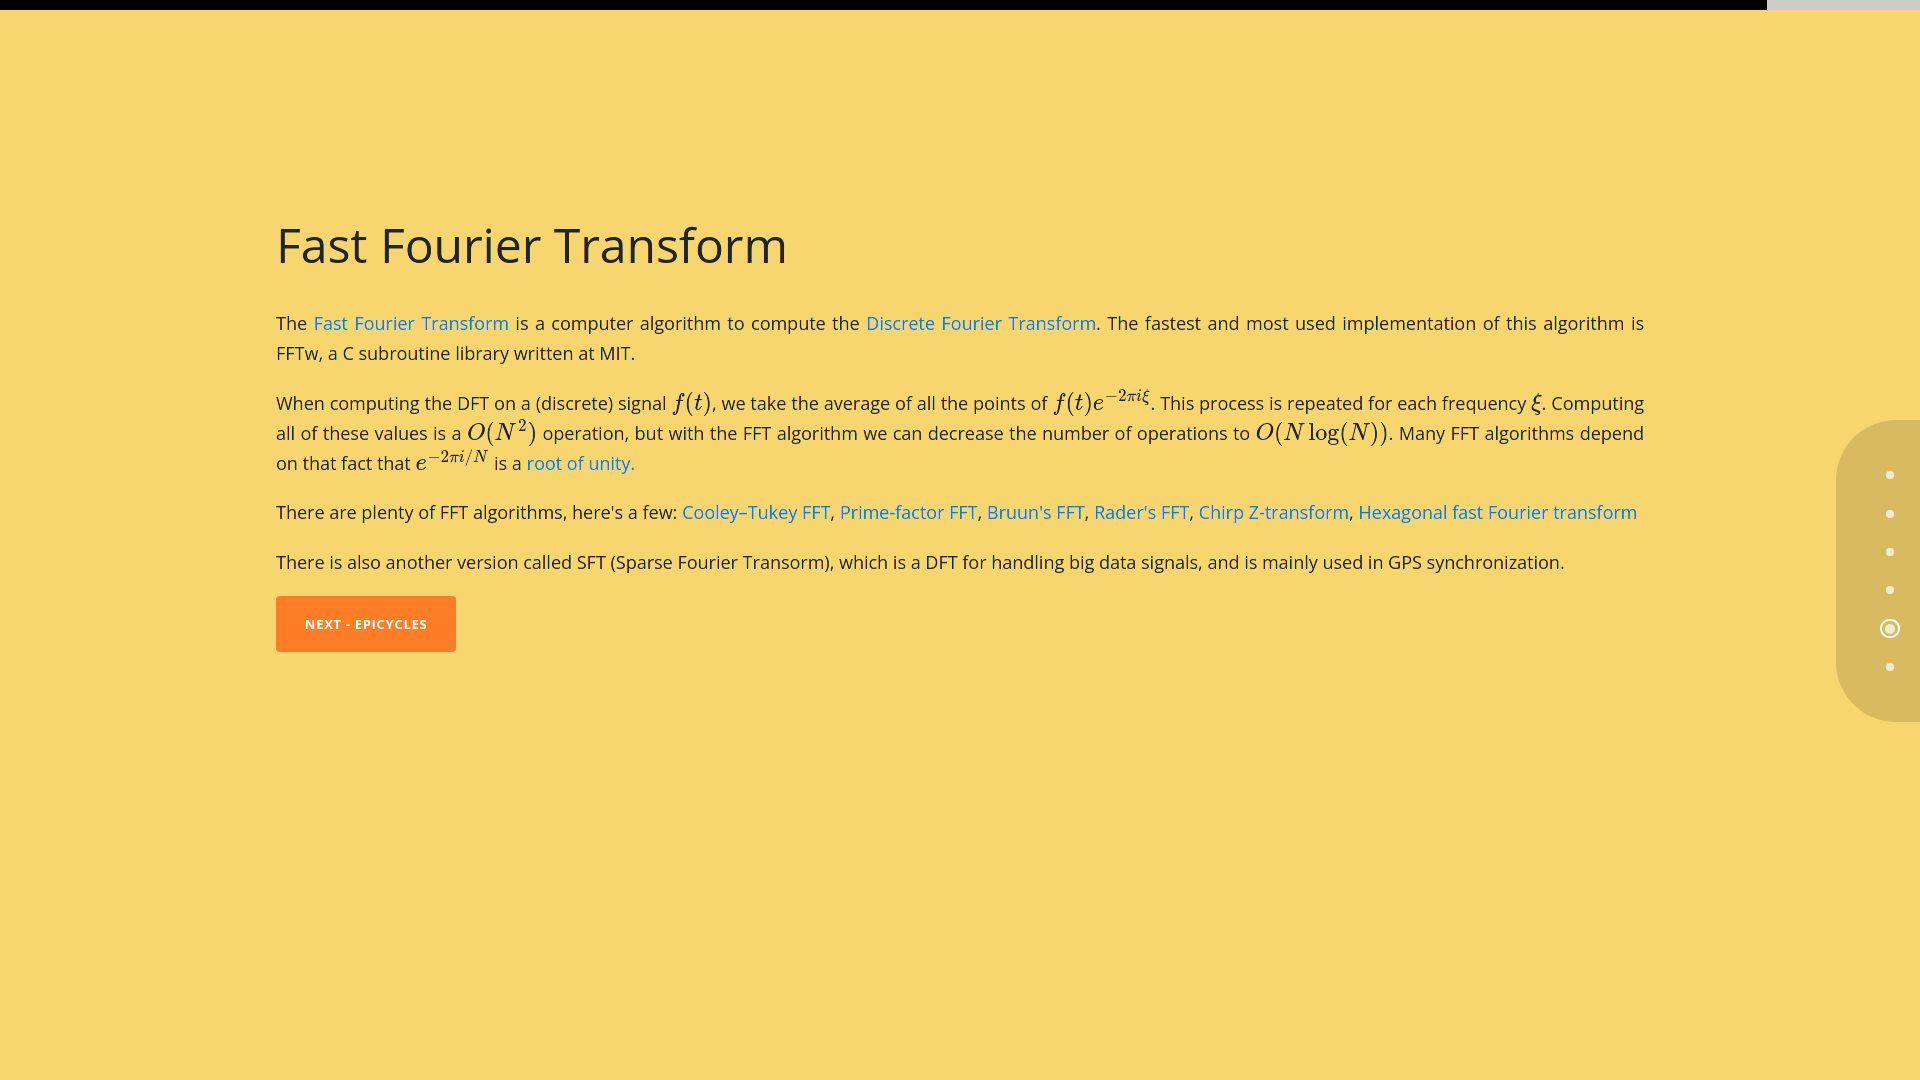
\includegraphics[width=\textwidth]{chap16.png}

\subsubsection{Epicycles}

How the animation in Chapter. 1 works.

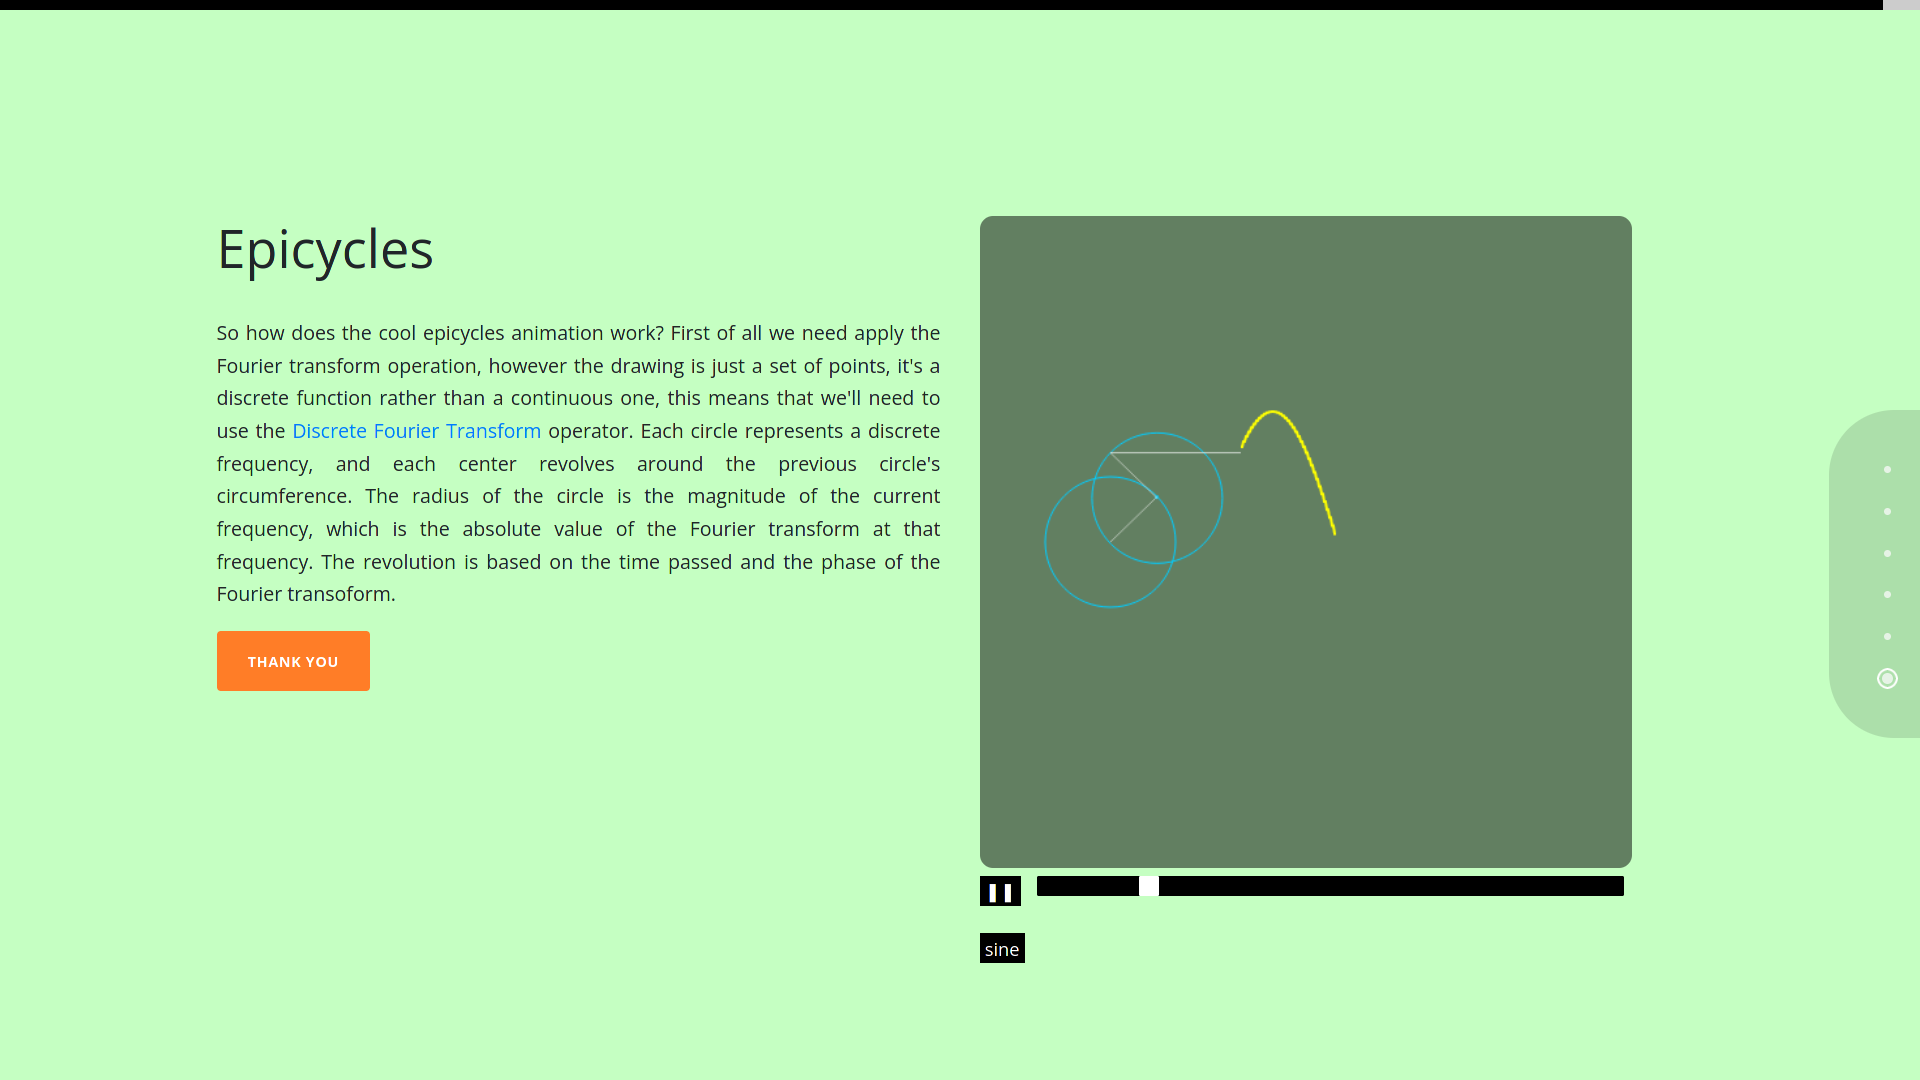
\includegraphics[width=\textwidth]{chap17.png}

\pagebreak

\subsection{Interactive Boxes Implementations}

\subsubsection{Fourier Series 1D}

\begin{multicols}{2}
    In order for this interactive box to work, the discrete Fourier transform
    of the signal must be computed, then, the result must be represented with epicycles.
    I wrote a function \texttt{dft(signal)} which computes the DFT and a function
    \texttt{drawEpicycles(ctx, dft, xOff, yOff, rot)} which draws a set of epicycles at a
    given point in the canvas space.
    Class name: \texttt{FourierSeries1D.js}.
    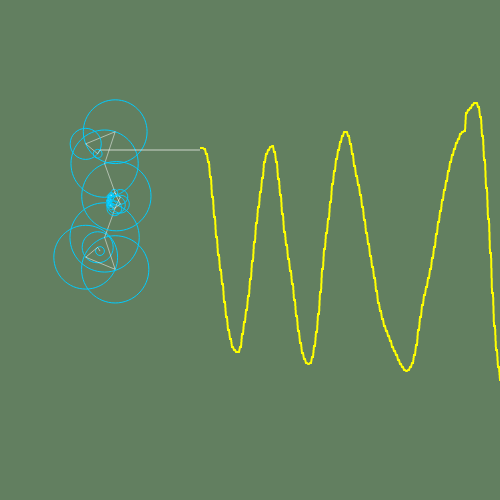
\includegraphics[width=0.5\textwidth]{fourierseries1d.png}
\end{multicols}

\subsubsection{Fourier Series 2D}

\begin{multicols}{2}
    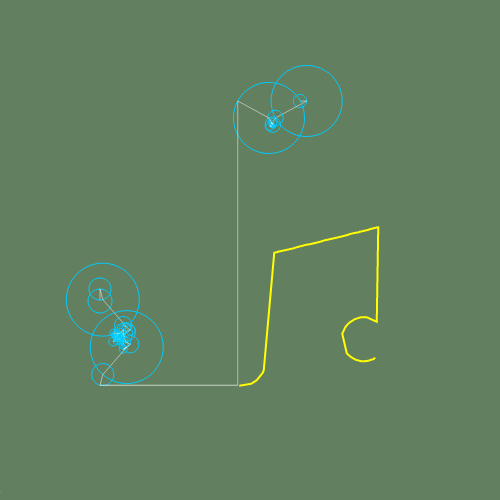
\includegraphics[width=0.5\textwidth]{fourierseries2d.png}
    This interactive box is basically the same as the previous one.
    The drawing is split into two signals: the \(x\)-coordinates and the \(y\)-coordinates.
    The discrete Fourier transform of the two signals is computed.
    Two sets of epicycles are drawn, one of which is rotated by \(\frac{\pi}{2}\).
    The conjunction of the two epicycles mix the signals and recreate the original drawing.
    Both the discrete Fourier transform and the function for drawing
    epicycles are recycled from the last interactive box.
    Class name: \texttt{FourierSeries2D.js}.
\end{multicols}

\pagebreak

\subsubsection{Complex Plot}

\begin{multicols}{2}
    This is the plot of the function \(f(t)e^{-2\pi it\xi}\).
    This interactive box also provides a slider for the frequency.
    A graph of the original signal is plotted at the top right corner.
    The signal around the origin is plotted using \(\sin\) and \(\cos\) coordinates.
    Class name: \texttt{ComplexPlot.js}.
    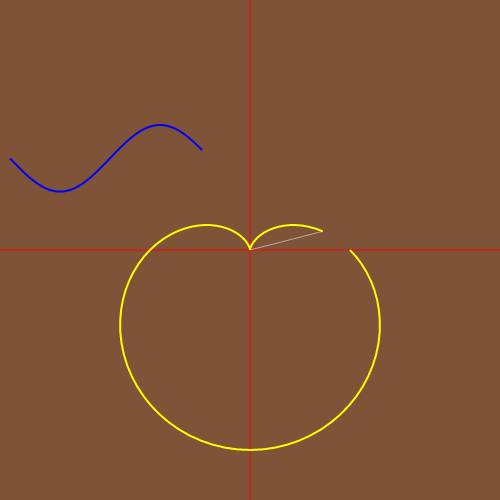
\includegraphics[width=0.5\textwidth]{complexplot.png}
\end{multicols}

\subsubsection{Center of Mass}

\begin{multicols}{2}
    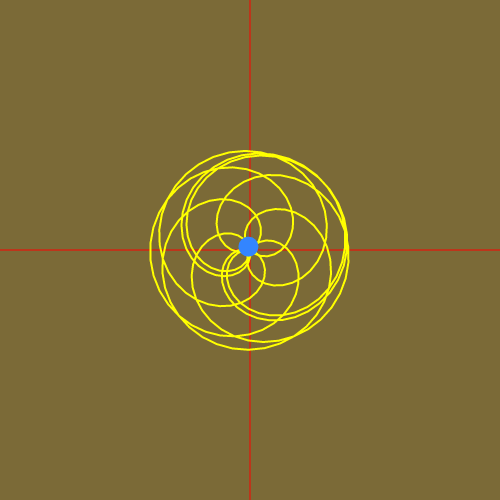
\includegraphics[width=0.5\textwidth]{centerofmass.png}
    This interactive box is similar to the last one.
    Instead of plotting the signal around the origin progressively over time,
    the full signal is plotted 3 times. The timeline doesn't represent
    the time anymore but rather the frequency. Whilst the animation is being drawn,
    the center of mass is computed and then represented with the blue dot.
    Class name: \texttt{CenterOfMass.js}.
\end{multicols}

\pagebreak

\subsubsection{Fourier Transform}

\begin{multicols}{2}
    For this interactive box a new implementation of the Discrete Fourier Transform
    is written. This new version specifically computes the DFT of a smaller range containing fractional frequencies.
    Class name: \texttt{FourierTransform.js}.
    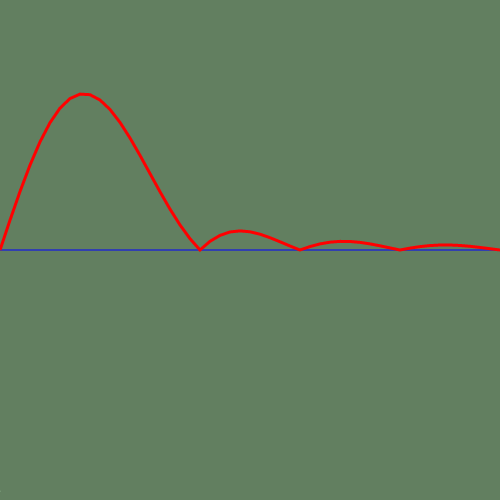
\includegraphics[width=0.5\textwidth]{fouriertransformabs.png}
\end{multicols}

\subsubsection{Common Traits}

All the implemented interactive boxes have a common trait. \\
When the users inputs any path, the coordinates are relative to the origin \((0,0)\)
of the canvas which is at the top-left corner. This means that there is always some
offset from the origin, and that the coordinates
lay on the first quadrant of the Cartesian plane.
This can cause visible issues since the interactive boxes are designed to work with a reasonably contained signal.
\\
To solve this problem, when the user inputs a path and the \texttt{setPoints(points)} function is called,
the leftmost or topmost point is computed, and then removed from each coordinate.
Some interactive boxes also compute the rightmost or lowest point to center the signal at \(x=0\)
(between the first and fourth quadrant in the Cartesian plane).
\\
However, I decided not to include this operation by default, since the programmer still
might want to use the actual coordinates from the canvas itself.

\pagebreak

\subsection{Desmos Integration}

Desmos is a graphing calculator. An API\cite{desmos} is provided to integrate the calculator in your website as follows:

Include the JavaScript file (a testing api key is provided on their website)

\begin{lstlisting}[style=html]
    <script src="https://www.desmos.com/api/v1.6/calculator.js?apiKey=dcb31709b452b1cf9dc26972add0fda6"></script>
\end{lstlisting}

Add an element to attach the calculator to

\begin{lstlisting}[style=html]
    <div id="calculator" style="width: 600px; height: 400px;"></div>
\end{lstlisting}

Attach the calculator to the element in a JavaScript environment

\begin{lstlisting}[style=js]
    var elt = document.getElementById('calculator');
    var calculator = Desmos.GraphingCalculator(elt);
    calculator.setExpression({ id: 'graph1', latex: 'y=x^2' });
\end{lstlisting}

\subsection{Template Integration}

I have chosen the template \texttt{tm-526-vanilla} from \href{https://templatemo.com}{templatemo.com}\cite{templatemo} for my website. \\
Little remains from the original template, I have kept and modified the following features:

\begin{itemize}
    \item The side navbar
    \item The section design
    \item The scroll button script
    \item The footer section
\end{itemize}

\pagebreak

\section{Testing}

\subsection{Test protocol}

\bgroup{}
\def\arraystretch{1.25}
\begin{center}
    \begin{tabular}{ |l|p{9cm}| }
        \hline
        \multicolumn{2}{|c|}{\textbf{Test-00}} \\
        \hline
        \textbf{Name} & Responsiveness \\
        \hline
        \textbf{Reference} & Req-02 \\
        \hline
        \textbf{Prerequisites} & The website must be open with a free internet connection using a modern browser on a mobile phone. \\
        \hline
        \textbf{Description} & Check if the website is readable and understandable and if all the features are preserved on a smaller monitor. \\
        \hline
    \end{tabular}
\end{center}
\egroup{}

\bgroup{}
\def\arraystretch{1.25}
\begin{center}
    \begin{tabular}{ |l|p{9cm}| }
        \hline
        \multicolumn{2}{|c|}{\textbf{Test-01}} \\
        \hline
        \textbf{Name} & Interactive Boxes \\
        \hline
        \textbf{Reference} & Req-03, Req-04 \\
        \hline
        \textbf{Prerequisites}
        & The website must be open with a free internet connection
        using a modern browser on a mobile phone. \\
        \hline
        \textbf{Description}
        & For each one of the interactive boxes,
        try to interact it with.
        The animation should respect what is explained in the section.
        Furthermore, the timeline, the play/pause button and the
        additional inputs (if present) should work properly. \\
        \hline
    \end{tabular}
\end{center}
\egroup{}

\subsection{Test results}

\bgroup{}
\def\arraystretch{1.25}
\begin{center}
    \begin{tabular}{ |l|l|l| }
        \hline
        \textbf{ID} & Result & Note \\
        \hline
        \textbf{Test-00} & \color{red} Failed & The website is bad formatted \\
        \hline
        \textbf{Test-01} & \color{darkgreen} Passed & All the interactive boxes work properly \\
        \hline
    \end{tabular}
\end{center}
\egroup{}

Req-01 has not been fulfilled. I have decided not to fulfill this requirement because of the lack
of support for canvases from mobile browsers. It is not possible to draw on canvases on any mobile
browser. Furthermore, some mobile browser don't even support them at all.
Even thought I used Bootstrap as my main CSS framework, which is prone to making responsive websites,
I decided that I would just be a waste of time, therefore, the website has been designed for a \(1920\times1080\) resolution only.

\pagebreak

\section{Conclusion}

\subsection{Further Development}

\subsubsection{Library Design}

Something that could be improved is OOP hierarchy. I could make
two classes extending \texttt{InteractiveBox.js}: \texttt{InteractiveBox1D.js} and
\texttt{InteractiveBox2D.js}. This way, every implementation of the library extends either
one of these two classes. The first one lets only the user draw a one-dimensional signal.
This is a problem in the current version, since some interactive boxes implementation only processes
the y-coordinate of the user drawn path, without blocking him from drawing a two-dimensional path.

\subsubsection{Website Content}

The website lacks of an explanation about the Fast Fourier Transform and how to implement it.
\\
Another covered topic could be the inverse Fourier operators.

\subsection{Personal Considerations}

I'm really happy with how the website turned out, and I've gained deep knowledge about Joseph Fourier's work.
However, I am dissatisfied with what I have written. There are so many topics concerning Fourier analysis and I wish I could have covered more.
\\
I think I managed the timing well, even though I finished later than expected.
\\
The nature of this project is very creative. At the beginning, I didn't have a precise picture of what I was going to
put on the website, I chose the content as I was studying the topic, but in the end I managed to almost respect my initial idea.

\pagebreak

\section{References}

\nocite{*} % cite all entries

\printbibliography[nottype=online, heading=subbibliography, title=Bibliography]
\printbibliography[type=online, heading=subbibliography, title=Sitography]

\end{document}

% compile:
% pdflatex documentation.tex;bibtex documentation;pdflatex documentation.tex;mv documentation.pdf ../